\documentclass[submission]{eptcs}
\providecommand{\event}{ACT 2023}

\usepackage[british]{babel}
\usepackage[utf8]{inputenc}
\usepackage[T1]{fontenc}

% Bibliography

%\usepackage[hyphen]{url}
\hypersetup{colorlinks, urlcolor=RoyalBlue, linkcolor=Red!80, citecolor=Green} % Needed to display links
\usepackage[hyphenbreaks]{breakurl}

%  Graphics
\usepackage{graphicx} % Needed to include images
%\usepackage{subcaption} % Needed to define subfigures
\usepackage[dvipsnames]{xcolor} % Needed to use color names in hyperref options

% Tikz
  \usepackage{tikz} % TikZ
  \usetikzlibrary{
    cd, % to make easy commutative diagrams
    petri, % To draw petri nets
    backgrounds, % To define image backgrounds
    arrows, % To use and define further arrow tips
    positioning, % To use expressions like "right = 1 of 1"
    decorations.markings, % Needed to define oriented wiring diagrams
    decorations.pathmorphing,
    calc,  % Needed to define oriented wiring diagrams
    fit, % Needed to compose wiring diagrams
    shapes.multipart
  }

% A TikZ style for curved arrows of a fixed height, due to AndréC.
\tikzset{curve/.style={settings={#1},to path={(\tikztostart)
    .. controls ($(\tikztostart)!\pv{pos}!(\tikztotarget)!\pv{height}!270:(\tikztotarget)$)
    and ($(\tikztostart)!1-\pv{pos}!(\tikztotarget)!\pv{height}!270:(\tikztotarget)$)
    .. (\tikztotarget)\tikztonodes}},
    settings/.code={\tikzset{quiver/.cd,#1}
        \def\pv##1{\pgfkeysvalueof{/tikz/quiver/##1}}},
    quiver/.cd,pos/.initial=0.35,height/.initial=0}

% TikZ arrowhead/tail styles.
\tikzset{tail reversed/.code={\pgfsetarrowsstart{tikzcd to}}}
\tikzset{2tail/.code={\pgfsetarrowsstart{Implies[reversed]}}}
\tikzset{2tail reversed/.code={\pgfsetarrowsstart{Implies}}}
% TikZ arrow styles.
\tikzset{no body/.style={/tikz/dash pattern=on 0 off 1mm}}

% Maths
\usepackage{mathtools} % Basic math capabilities
\usepackage{amssymb} % Extra mathematical symbols (loads amsfonts)
\usepackage{dsfont}
\usepackage{mathrsfs}
\let\proof\relax
\let\endproof\relax
\usepackage{amsthm} % Theorem environments
\usepackage{stmaryrd} % Some maths symbols for logic and computer science

%% WRITING %%
\usepackage{relsize} % Additional relative sizes for fonts
\usepackage{microtype} % Improves appearance of writing
\usepackage{multicol} % Multi-column environments
\usepackage{csquotes} % Environments for quotes
\usepackage{xspace}
\usepackage{enumitem}
\usepackage{fontawesome} % Popular fontawesome symbols

% List of Symbols
\usepackage{tabularx, cellspace} % Needed to typeset the tables for listing symbols
\setlength\cellspacetoplimit{3pt}
\setlength\cellspacebottomlimit{3pt}
% David's
\usepackage[capitalize]{cleveref}

\usepackage{datetime}

% Theorem Environments
%
% Theorem Counters
%
\newcounter{theoremUnified} % Unified coutner for all theorem environments
\def\thetheoremUnified{\arabic{section}} % Needed to have counters going with sections
\numberwithin{theoremUnified}{section} % Numbering within sections
\numberwithin{theoremUnified}{section} % Equations are also numbered within sections

% Theorem Styles
%
\newtheoremstyle{plainStyle} % Plain theorem style
	{2mm} % Space above
	{2mm} % Space below
	{} % Body font
	{} % Indent amount
	{\bfseries} % Theorem head font
	{.} % Punctuation after theorem head
	{.5em} % Space after theorem head
	{} % Theorem head spec (can be left empty, meaning `normal')

\newtheoremstyle{italicStyle} % Italic theorem style
	{2mm} % Space above
	{2mm} % Space below
	{\itshape} % Body font
	{} % Indent amount
	{\bfseries} % Theorem head font
	{.} % Punctuation after theorem head
	{.5em} % Space after theorem head
	{} % Theorem head spec (can be left empty, meaning `normal')

% Environments
\theoremstyle{plainStyle}
	\newtheorem{notation}{Notation}{\rmfamily}{\rmfamily}
	\newtheorem{definition}{Definition}{\rmfamily}{\rmfamily}
	\newtheorem{remark}{Remark}{\rmfamily}{\rmfamily}
	\newtheorem{example}{Example}{\rmfamily}{\rmfamily}
	\newtheorem{counterexample}{Counterexample}{\rmfamily}{\rmfamily}

\theoremstyle{italicStyle}
	\newtheorem{proposition}{Proposition}{\rmfamily}{\rmfamily}
	\newtheorem{theorem}{Theorem}{\rmfamily}{\rmfamily}
	\newtheorem{corollary}{Corollary}{\rmfamily}{\rmfamily}

\relpenalty=10000
\binoppenalty=10000
\setlength\parindent{1em}

% Autoref styling
% Capitalize references
    \renewcommand{\chapterautorefname}{Chapter}
    \renewcommand{\sectionautorefname}{Section}
    \renewcommand{\theoremautorefname}{Theorem}
    \renewcommand{\chapterautorefname}{Chapter}
    \renewcommand{\sectionautorefname}{Section}
% Refer to sub- and subsubsections as 'section'
    \let\subsectionautorefname\sectionautorefname
    \let\subsubsectionautorefname\sectionautorefname
% Give a name to new environments
    \newcommand{\notationautorefname}{Notation}
    \newcommand{\definitionautorefname}{Definition}
    \newcommand{\propositionautorefname}{Proposition}
    \newcommand{\remarkautorefname}{Remark}
    \newcommand{\exampleautorefname}{Example}
    \newcommand{\counterexampleautorefname}{Counterexample}
    \newcommand{\corollaryautorefname}{Corollary}
% Macros shared among templates

\usepackage[utf8]{inputenc}

\usepackage{graphicx}
\setkeys{Gin}{width=\linewidth,totalheight=\textheight,keepaspectratio}

\definecolor{darkblue}{HTML}{00416A}

\usepackage{longtable}
\usepackage{booktabs}
\usepackage{amssymb}
\usepackage{amsmath}
\usepackage{amsthm}
%\usepackage{commath}
\usepackage{boxedminipage}
\usepackage{microtype}

\usepackage{makeidx}
\usepackage{hyperref}

% attempts to prevent margin figures from being cut off
\usepackage{marginfix}
\usepackage[morefloats=100]{morefloats}

\newtheorem{Definition}{Definition}
\newtheorem{Theorem}{Theorem}
\newtheorem{Lemma}{Lemma}
\newtheorem{Exercise}{Exercise}
\newtheorem{Fact}{Fact}
\newtheorem{Proposition}{Proposition}
\newtheorem{Assumption}{Assumption}
\newenvironment{Algorithm}{\begin{center}\begin{boxedminipage}{0.92\textwidth}}{\end{boxedminipage}\end{center}}
\newenvironment{Proof}{\begin{proof}}{\end{proof}}
\newtheorem*{summary*}{Summary}
\newenvironment{Summary}{\begin{center}\begin{minipage}{0.92\textwidth}\begin{summary*}}{\end{summary*}\end{minipage}\end{center}\medskip}
\newenvironment{EmphBox}{\begin{center}\begin{minipage}{0.8\textwidth}}{\end{minipage}\end{center}\medskip}

\providecommand{\tightlist}{%
  \setlength{\itemsep}{0pt}\setlength{\parskip}{0pt}}

\renewcommand{\bot}{\perp}
\renewcommand{\hat}{\widehat}


% Ubiquitous set names
%
\newcommand{\Naturals}{\mathbb{N}} % Set of natural numbers
\newcommand{\Integers}{\mathbb{Z}} % Set of interer numbers
\newcommand{\Complex}{\mathbb{C}}  % Set of complex numbers

% Basic Definitions
%
\newcommand{\Cp}{\fatsemi} % Morphism composition in diagrammatic order

\DeclareMathOperator{\Obj}{Obj}%[1]{\operatorname{Obj} \, #1} % Set of objects of category #1
\DeclareMathOperator{\Mor}{Mor}%[1]{\operatorname{Mor} \, #1} % Set of objects of category #1
\DeclareMathOperator{\GObj}{GObj}%[1]{\operatorname{GenObj} \, #1} % Set of objects of category #1
\DeclareMathOperator{\GMor}{GMor}%[1]{\operatorname{GenMor} \, #1} % Set of objects of category #1

\newcommand{\Homtotal}[1]{\operatorname{Hom}_{\,#1}} % Set of morphisms of category #1
\newcommand{\Hom}[3]{\operatorname{Hom}_{\,#1}\left[#2,#3\right]} % Set of morphisms of category #1 from object #2 to object #3
\newcommand{\Source}[1]{\operatorname{s}(#1)} % Domain of function/morphism #1
\newcommand{\Target}[1]{\operatorname{t}(#1)} % Domain of function/morphism #1
\newcommand{\Id}[1]{\text{id}_{#1}} % Identity morphism of object #1
\newcommand{\Op}[1]{{#1}^{\text{op}}} % op functor

% Generic names for categories
%
\newcommand{\CategoryA}{\mathit{A}}
\newcommand{\CategoryB}{\mathit{B}}
\newcommand{\CategoryC}{\mathit{C}}
\newcommand{\CategoryD}{\mathit{D}}
\newcommand{\CategoryE}{\mathit{E}}

\newcommand{\WTerm}{\mathds{1}}
\newcommand{\Term}{\mathbf{1}}

% Category names    
%
\newcommand{\Set}{\mathbf{Set}} % Category of sets and functions
\newcommand{\SetS}{{\Set_{*}}} % Category of sets and functions
\newcommand{\Hask}{\mathbf{Hask}} % Category of data types and Haskell functions
\newcommand{\Group}{\mathbf{Group}} % Category of groups and homomorphisms
\newcommand{\Top}{\mathbf{Top}} % Category of topological spaces and continuous functions
\newcommand{\Rel}{\mathbf{Rel}} % Category of sets and relations
\newcommand{\Span}{\mathbf{Span}} % Category of sets and spans
\newcommand{\hTop}{\mathbf{hTop}} % Category of topological spaces and homotopy classes of continuous functions
\newcommand{\Cat}{\mathbf{Cat}} % Category of categories

% Monoidal Categories
%
\newcommand{\Tensor}{\otimes} % Monoidal tensor
\newcommand{\TensorUnit}{I} % Monoidal tensor unit


% Logic
%
\newcommand{\Suchthat}[2]{\left\{#1 \: \middle\vert \: #2\right\}} % Set of elements #1 such that condition #2 holds 

\usepackage[papersize={6.6in, 10.0in}, left=.5in, right=.5in, top=.6in, bottom=.9in]{geometry}
\linespread{1.05}
\sloppy
\raggedbottom
\pagestyle{plain}

\hypersetup{
breaklinks=true
,urlcolor=blue
,anchorcolor=blue
,citecolor=blue
,filecolor=blue
,linkcolor=blue
,menucolor=blue
,linktocpage=true]{hyperref}
bookmarksopen=true,
bookmarksnumbered=true,
bookmarksopenlevel=10
}
% these include amsmath and that can cause trouble in older docs.
\input{../helpers/cmrsum}
\makeatletter

\DeclareFontFamily{OMX}{MnSymbolE}{}
\DeclareSymbolFont{largesymbolsX}{OMX}{MnSymbolE}{m}{n}
\DeclareFontShape{OMX}{MnSymbolE}{m}{n}{
    <-6>  MnSymbolE5
   <6-7>  MnSymbolE6
   <7-8>  MnSymbolE7
   <8-9>  MnSymbolE8
   <9-10> MnSymbolE9
  <10-12> MnSymbolE10
  <12->   MnSymbolE12}{}

\DeclareMathSymbol{\downbrace}    {\mathord}{largesymbolsX}{'251}
\DeclareMathSymbol{\downbraceg}   {\mathord}{largesymbolsX}{'252}
\DeclareMathSymbol{\downbracegg}  {\mathord}{largesymbolsX}{'253}
\DeclareMathSymbol{\downbraceggg} {\mathord}{largesymbolsX}{'254}
\DeclareMathSymbol{\downbracegggg}{\mathord}{largesymbolsX}{'255}
\DeclareMathSymbol{\upbrace}      {\mathord}{largesymbolsX}{'256}
\DeclareMathSymbol{\upbraceg}     {\mathord}{largesymbolsX}{'257}
\DeclareMathSymbol{\upbracegg}    {\mathord}{largesymbolsX}{'260}
\DeclareMathSymbol{\upbraceggg}   {\mathord}{largesymbolsX}{'261}
\DeclareMathSymbol{\upbracegggg}  {\mathord}{largesymbolsX}{'262}
\DeclareMathSymbol{\braceld}      {\mathord}{largesymbolsX}{'263}
\DeclareMathSymbol{\bracelu}      {\mathord}{largesymbolsX}{'264}
\DeclareMathSymbol{\bracerd}      {\mathord}{largesymbolsX}{'265}
\DeclareMathSymbol{\braceru}      {\mathord}{largesymbolsX}{'266}
\DeclareMathSymbol{\bracemd}      {\mathord}{largesymbolsX}{'267}
\DeclareMathSymbol{\bracemu}      {\mathord}{largesymbolsX}{'270}
\DeclareMathSymbol{\bracemid}     {\mathord}{largesymbolsX}{'271}

\def\horiz@expandable#1#2#3#4#5#6#7#8{%
  \@mathmeasure\z@#7{#8}%
  \@tempdima=\wd\z@
  \@mathmeasure\z@#7{#1}%
  \ifdim\noexpand\wd\z@>\@tempdima
    $\m@th#7#1$%
  \else
    \@mathmeasure\z@#7{#2}%
    \ifdim\noexpand\wd\z@>\@tempdima
      $\m@th#7#2$%
    \else
      \@mathmeasure\z@#7{#3}%
      \ifdim\noexpand\wd\z@>\@tempdima
        $\m@th#7#3$%
      \else
        \@mathmeasure\z@#7{#4}%
        \ifdim\noexpand\wd\z@>\@tempdima
          $\m@th#7#4$%
        \else
          \@mathmeasure\z@#7{#5}%
          \ifdim\noexpand\wd\z@>\@tempdima
            $\m@th#7#5$%
          \else
           #6#7%
          \fi
        \fi
      \fi
    \fi
  \fi}

\def\overbrace@expandable#1#2#3{\vbox{\m@th\ialign{##\crcr
  #1#2{#3}\crcr\noalign{\kern2\p@\nointerlineskip}%
  $\m@th\hfil#2#3\hfil$\crcr}}}
\def\underbrace@expandable#1#2#3{\vtop{\m@th\ialign{##\crcr
  $\m@th\hfil#2#3\hfil$\crcr
  \noalign{\kern2\p@\nointerlineskip}%
  #1#2{#3}\crcr}}}

\def\overbrace@#1#2#3{\vbox{\m@th\ialign{##\crcr
  #1#2\crcr\noalign{\kern2\p@\nointerlineskip}%
  $\m@th\hfil#2#3\hfil$\crcr}}}
\def\underbrace@#1#2#3{\vtop{\m@th\ialign{##\crcr
  $\m@th\hfil#2#3\hfil$\crcr
  \noalign{\kern2\p@\nointerlineskip}%
  #1#2\crcr}}}

\def\bracefill@#1#2#3#4#5{$\m@th#5#1\leaders\hbox{$#4$}\hfill#2\leaders\hbox{$#4$}\hfill#3$}

\def\downbracefill@{\bracefill@\braceld\bracemd\bracerd\bracemid}
\def\upbracefill@{\bracefill@\bracelu\bracemu\braceru\bracemid}

\DeclareRobustCommand{\downbracefill}{\downbracefill@\textstyle}
\DeclareRobustCommand{\upbracefill}{\upbracefill@\textstyle}

\def\upbrace@expandable{%
  \horiz@expandable
    \upbrace
    \upbraceg
    \upbracegg
    \upbraceggg
    \upbracegggg
    \upbracefill@}
\def\downbrace@expandable{%
  \horiz@expandable
    \downbrace
    \downbraceg
    \downbracegg
    \downbraceggg
    \downbracegggg
    \downbracefill@}

\DeclareRobustCommand{\overbrace}[1]{\mathop{\mathpalette{\overbrace@expandable\downbrace@expandable}{#1}}\limits}
\DeclareRobustCommand{\underbrace}[1]{\mathop{\mathpalette{\underbrace@expandable\upbrace@expandable}{#1}}\limits}

\makeatother


\setcounter{tocdepth}{2}
%
%
\begin{document}
    \title{Obstructions to Compositionality}

    \author{        
        Caterina Puca
            %\email{OrcID here}
            \institute{Quantinuum\textsuperscript{*}}
            \email{caterina.puca@quantinuum.com}
        \and
        Amar Hadzihasanovic
            %\email{OrcID here}
            \institute{$^1$ Quantinuum\textsuperscript{*} \\$^2$ Tallinn University of Technology}%\footref{note: Quantinuum Address}}
            \email{amar.hadzihasanovic@quantinuum.com}
        \and
        Fabrizio Genovese
            %\email{OrcID here}
            \institute{20squares}
            \email{noreply@20squares.xyz}
        \and
        Bob Coecke
            %\email{OrcID here}
            \institute{Quantinuum\footnote{17 Beaumont Street, Oxford OX1 2NA, United Kingdom}}
            \email{bob.coecke@quantinuum.com}
    }

    \def\titlerunning{Obstructions to Compositionality}
    \def\authorrunning{Puca, Hadzihasanovic, Genovese, Coecke}

    \maketitle
    \begin{abstract}

Compositionality is at the heart of computer science and several other areas of applied category theory such as computational linguistics, categorical quantum mechanics, interpretable AI, dynamical systems, compositional game theory, and Petri nets. 
However, the meaning of the term seems to vary across the many different applications.
This work contributes to understanding, and in particular qualifying, different kinds of compositionality.

Formally, we introduce invariants of categories that we call zeroth and first homotopy posets, generalising in a precise sense the $\pi_0$ and $\pi_1$ of a groupoid.
These posets can be used to obtain a qualitative description of how far an object is from being terminal and a morphism is from being iso.
In the context of applied category theory, this formal machinery gives us a way to qualitatively describe the ``failures of compositionality'', seen as failures of certain (op)lax functors to be strong, by classifying obstructions to the (op)laxators being isomorphisms. 

Failure of compositionality, for example for the interpretation of a categorical syntax in a semantic universe, can both be a bad thing and a good thing, which we illustrate by respective examples in graph theory and quantum theory.

    \end{abstract}
    %
    \paragraph*{\bf Acknowledgements}
    %
        A.H.\ was supported by the ESF funded Estonian IT Academy research measure (project 2014-2020.4.05.19-0001) and by the Estonian Research Council grant PSG764.
        We thank Sean Tull and Robin Lorenz for helpful comments on an earlier draft.

    
\section{Introduction \label{sec:introduction}}

When probed at very short wavelengths, QCD is essentially a theory of
free \index{Partons}`partons' --- quarks and gluons --- which only
scatter off one another through relatively small quantum corrections,
that can be systematically calculated. 
But at longer wavelengths, of order the size of the proton $\sim
1\mathrm{fm} = 10^{-15}\mathrm{m}$,  
we see strongly bound towers of hadron resonances emerge, with string-like
potentials building up if we try to separate their partonic
constituents. Due to our
inability to perform analytic calculations in 
strongly coupled field theories, QCD is therefore 
still only partially solved. Nonetheless,  all its features, across all
distance scales, are believed to be encoded in a single one-line
formula of alluring simplicity; the
\index{QCD!Lagrangian}%
Lagrangian\footnote{Throughout these notes we let it be implicit that
  ``Lagrangian'' really refers to Lagrangian density, ${\cal L}$, the
  four-dimensional space-time integral of which is the action.} of QCD.

The consequence for collider physics is that some parts of QCD can be
calculated in terms of the fundamental parameters of the Lagrangian,
whereas others must be expressed through models or functions whose effective 
parameters are not a priori calculable but which can be constrained
by fits to data. 
However, even in the absence of a
perturbative expansion, there are still several strong theorems which
hold, and which can be used to give relations between seemingly
different processes. (This is, e.g., the reason it makes sense to 
measure the partonic substructure of the proton in $ep$ collisions and
then re-use the same parametrisations for $pp$
collisions.) Thus, in the chapters 
dealing with phenomenological models we shall emphasise that the loss
of a factorised perturbative expansion is not equivalent to a total
loss of predictivity.   

An alternative approach would be to give up on calculating QCD 
and use leptons instead. Formally, this amounts to summing inclusively over
strong-interaction phenomena, when such are present. While such a
strategy might succeed in replacing what we do know about QCD by
``unity'', however, even the most adamant chromophobe would acknowledge
the following basic facts of collider physics for the next decade(s): 
1) At the LHC, the initial states are
hadrons, and hence, at
the very least, well-understood and precise parton distribution
functions (PDFs) will be required; 2) high precision will mandate
 calculations to higher orders in perturbation theory, 
which in turn will involve more QCD; 3) the requirement of lepton
\emph{isolation} makes the very definition of a lepton
 depend implicitly on QCD and 4) 
 the rate of jets that are misreconstructed as leptons in
 the experiment depends explicitly on it. 
And, 5) though many new-physics signals \emph{do} give observable
signals in the lepton sector, this is far from guaranteed, nor is it
exclusive when it occurs. 
 It would therefore be  unwise not to attempt to solve QCD to the best
 of our ability, the better to prepare ourselves for both the largest
 possible discovery reach and the highest attainable subsequent
 precision. 

Furthermore, QCD is the richest gauge theory we have so far
 encountered. Its emergent phenomena, unitarity properties, colour structure, 
 non-perturbative dynamics, quantum vs.\ classical limits, 
interplay between scale-invariant and
 scale-dependent properties, and its wide
 range of phenomenological applications, are still very much topics of
 active investigation, about which we continue to learn.  

In addition, or perhaps as a consequence, the field of QCD is
currently experiencing something of a revolution. On the perturbative
side, new methods to compute scattering amplitudes with very high
particle multiplicities are being developed, together with advanced
techniques for combining such amplitudes with all-orders resummation
frameworks. On the non-perturbative side, the wealth of data on
soft-physics processes from the LHC is
forcing us to reconsider the reliability of the standard fragmentation
models, and heavy-ion collisions are providing new insights into
the collective behavior of hadronic matter. The
study of cosmic rays impinging on the Earth's
atmosphere challenges our ability to extrapolate fragmentation models
from collider energy scales to the region of ultra-high energy cosmic
rays. And finally, dark-matter annihilation processes in space  may produce 
hadrons, whose spectra are sensitive to the modeling 
of fragmentation.

In the following, we shall focus on QCD for mainstream 
collider physics. This includes the basics of SU(3), colour factors, the running
of $\alpha_s$, factorisation, 
hard processes, infrared safety, parton showers and matching, event generators, hadronisation, and the so-called underlying event. 
While not covering everything, hopefully these topics can also serve
at least as stepping stones to more specialised
issues that have been left out, such as twistor-inspired techniques, 
heavy flavours, polarisation, or forward physics, or to topics more tangential to
other fields, such as axions, lattice QCD, or heavy-ion physics.  

\subsection{A First Hint of Colour}
Looking for new physics, as we do now at the LHC, it is instructive to 
consider the story of the discovery of colour. The first hint was
arguably the $\Delta^{++}$ \index{Baryons}baryon, discovered in 
1951~\cite{Brueckner:1952zz}. The title and part of the abstract from this
historical paper are reproduced in \figRef{fig:Delta}.
\begin{figure}[t]
\begin{center}
\begin{tabular}{c}
\colorbox{gray}{\includegraphics*[scale=0.75]{DeltaTitle.pdf}}\\[5mm]
\hspace*{2mm}\begin{minipage}{0.88\textwidth}
\small\sl  ``[...] It is concluded that the apparently anomalous features of the
scattering can be interpreted to be an indication of a resonant
meson-nucleon interaction corresponding to a nucleon isobar with spin
$\frac32$, isotopic spin $\frac32$, and with an excitation energy of
$277\,$MeV.''\\[1mm]
\end{minipage}
\end{tabular}
\caption{The title and part of the abstract of the 1951 paper
  \cite{Brueckner:1952zz} (published in 1952) in which the existence 
  of the $\Delta^{++}$ baryon was deduced, based on data from Sachs and
  Steinberger at Columbia~\cite{Chedester:1951sc}  and from Anderson,
  Fermi, Nagle, et al.~at Chicago~\cite{Fermi:1952zz}. Further studies 
  at Chicago were quickly performed
  in~\cite{Anderson:1952nw,Anderson:1952zza}. See also the memoir by
  Nagle~\cite{nagle1984delta}. 
\label{fig:Delta}}  
\end{center}
\end{figure}
In the context of the \index{Quarks}quark model --- which first
had to be developed, successively joining together the notions of 
spin, isospin, strangeness, and 
the \index{Eightfold way}eightfold way\footnote{In physics, the ``eightfold way''
refers to the classification of the lowest-lying pseudoscalar
\index{Mesons}mesons and 
\index{SU(3)!Of Flavour}%
spin-1/2 \index{Baryons}baryons within \index{Octet}octets in SU(3)-flavour space ($u,d,s$). The
$\Delta^{++}$ is part of a spin-3/2 baryon \index{Decuplet}decuplet, a ``tenfold way'' in this
terminology.} 
--- the \index{Flavour}flavour and spin content of the $\Delta^{++}$
baryon is: 
\begin{equation}
\left\vert \Delta^{++} \right> = \left\vert
\,u_\uparrow\ u_\uparrow\ u_\uparrow \right>~,
\end{equation} 
clearly a highly symmetric configuration. However, since 
the $\Delta^{++}$ is a fermion, it must have an overall
antisymmetric wave function. In 1965, fourteen years after its
discovery, this was finally understood by the introduction of colour
\index{SU(3)}%
\index{SU(3)!Of Colour}%
as a new quantum number associated with the group SU(3)
\cite{Greenberg:1964pe,Han:1965pf}. The $\Delta^{++}$ wave function can now be made
antisymmetric by arranging its three quarks antisymmetrically 
in this new degree of freedom, 
\begin{equation}
\left\vert \Delta^{++} \right> = \epsilon^{ijk} \left\vert
\,u_{i\uparrow}\ u_{j\uparrow}\ u_{k\uparrow}\right>~,
\end{equation} 
hence solving the mystery.

More direct experimental tests of the number of colours were provided first by
measurements of the decay width of $\pi^0\to \gamma\gamma$ decays, which 
is proportional to $N_C^2$, 
and later by the famous ``R'' ratio in
$e^+e^-$ collisions ($R=\sigma(e^+e^-\to q\bar{q})/\sigma(e^+e^-\to
\mu^+\mu^-)$), which is proportional to $N_C$, see
e.g.~\cite{Dissertori:2003pj}. 
Below, in \SecRef{sec:L} we shall see how to
calculate such colour factors. 

\subsection{The Lagrangian of QCD \label{sec:L}}
\index{QCD!Lagrangian}%
Quantum Chromodynamics is based on the gauge group
\index{SU(3)}$\mrm{SU(3)}$, the 
Special Unitary group in 3 (complex) dimensions, whose elements 
are the set of unitary $3\times 3$ matrices with determinant one. 
\index{Fundamental representation}%
\index{SU(3)!Fundamental representation}%
Since there are 9 linearly independent unitary complex
matrices\footnote{A complex $N\times N$ matrix has $2N^2$ degrees of
  freedom, on which unitarity provides $N^2$ constraints.}, one of
which has determinant $-1$, there are a total of 8
independent directions in this matrix space, corresponding to eight
different generators as compared
with the single one of QED. In the context of QCD, we normally
represent this group using the 
so-called \emph{fundamental}, or \emph{defining}, representation, in
which the generators of $\mrm{SU(3)}$ appear as a set of eight traceless and
hermitean matrices, to which we return below.  
We shall refer to indices enumerating
the rows and columns of these matrices  (from 1 to 3) as
\emph{fundamental} indices, and we use the letters $i$,
$j$, $k$, \ldots, to denote them.
\index{Adjoint representation}%
\index{SU(3)!Adjoint representation}%
We refer to indices enumerating the generators (from 1 to 8),
as \emph{adjoint} 
indices\footnote{The dimension of the \emph{adjoint}, or
  \emph{vector}, representation is equal to the number of generators,
  $N^2-1=8$ for $\mrm{SU(3)}$, while the  
\index{Fundamental representation}%
\index{SU(3)!Fundamental representation}%
dimension of the fundamental representation is
  the degree of the group, $N=3$ for $\mrm{SU(3)}$.}, and we use the first
letters of the alphabet ($a$, $b$, $c$, \ldots) to denote them. 
These matrices can operate both on each other (representing
combinations of successive gauge transformations) and on a set of
$3$-vectors, the latter of 
which represent \index{Quarks}quarks in colour 
space; the quarks are \emph{triplets} under $\mrm{SU(3)}$. The matrices can be
thought of as representing gluons in colour 
space (or, more precisely, the gauge transformations carried out by
gluons), hence there are
eight different gluons; the gluons are \emph{octets} under $\mrm{SU(3)}$. 

\index{QCD!Lagrangian}%
The Lagrangian density of QCD is 
\begin{equation}
{\cal L} = \bar{\psi}_q^i(i\gamma^\mu)(D_\mu)_{ij}\psi_q^j - m_q
\bar{\psi}_q^i\psi_{qi} - \frac14 F^a_{\mu\nu}F^{a\mu\nu}~,\label{eq:L}
\end{equation}
where $\psi_q^i$ denotes a quark field with
(fundamental) colour index $i$, 
$\psi_q = ({\textcolor{red}{\psi_{qR}}},{\color{green}\psi_{qG}}, 
{\color{blue}\psi_{qB}})^T$, 
$\gamma^\mu$ is a Dirac matrix that expresses the
vector nature of the strong interaction, with $\mu$ being a Lorentz
vector index, $m_q$ allows for the
possibility of non-zero \index{Quarks}quark masses (induced by the
standard Higgs 
mechanism or similar), $F^a_{\mu\nu}$ is the gluon field strength 
tensor for a gluon\footnote{The definition of the gluon field strength
  tensor will be given below in \eqRef{eq:F}.} with (adjoint) 
colour index $a$ (i.e., $a\in[1,\ldots,8]$), 
and $D_\mu$ is the covariant derivative in QCD,
\begin{equation}
(D_{\mu})_{ij} = \delta_{ij}\partial_\mu - i g_s t_{ij}^a A_\mu^a~,\label{eq:D}
\end{equation}
\index{QCD!Coupling}
with $g_s$ the \index{alphaS@$\alpha_s$}strong coupling (related to
$\alpha_s$ by $g_s^2 = 4\pi 
\alpha_s$; we return to the strong coupling in more detail below), 
$A^a_\mu$  the gluon field with 
colour index $a$, and $t_{ij}^a$ proportional to the hermitean and
traceless \index{Gell-Mann matrices|see{SU(3)}}Gell-Mann matrices of $\mrm{SU(3)}$, 
\index{SU(3)!Generators}%
\begin{equation}
\mbox{\includegraphics*[scale=1.0]{gell-mann}}~.
\end{equation}
These generators are just the $\mrm{SU(3)}$ analogs of the
Pauli matrices in 
$\mrm{SU(2)}$. 
By convention, the constant of proportionality is normally
taken to 
be 
\begin{equation}
t^a_{ij} = \frac12 \lambda^a_{ij}~. \label{eq:t}
\end{equation}
\index{QCD!Coupling}
This choice in turn determines the normalisation of the coupling
$g_s$, via \eqRef{eq:D}, and
fixes the values of the $\mrm{SU(3)}$ \index{Casimirs}Casimirs and structure constants, to which we return below. 

An example of the colour flow for a
quark-gluon interaction in colour 
space is given in \figRef{fig:qg}.
\begin{figure}[t]
\begin{center}
\begin{minipage}[h]{4.6cm}
\begin{center}
$A^1_\mu$\\
\includegraphics*[scale=0.75]{qgv.pdf}\\[-3mm]
$\psi_{q\textcolor{green}{G}}$\hfill$\psi_{q\textcolor{red}{R}}$
\end{center}
\end{minipage}~~~
\parbox{0.4\textwidth}{
$
\begin{array}{ccccc}
\propto & - \frac{i}{2} g_s & \bar{\psi}_{q\color{red}R}  & \lambda^{1} & \psi_{q\color{green}G} 
\\[2mm]
= & -\frac{i}{2}g_s & \left(\begin{array}{ccc} \textcolor{red}{1} & \color{green} 0 &
  \color{blue} 0 
\end{array}\right) & 
\left(\begin{array}{ccc}
0 & 1 & 0  \\
1 & 0 & 0 \\
0 & 0 & 0
\end{array}\right) & 
 \left(\begin{array}{c}
\textcolor{red}{0} \\
\color{green}1 \\
\color{blue}0
\end{array}\right) \end{array}
$}
\caption{Illustration of a 
\index{Quarks}\index{Gluons}$qqg$ vertex in QCD, before
  summing/averaging over colours: a gluon in a state represented by $\lambda^1$
  interacts with quarks in the states $\psi_{qR}$ and
  $\psi_{qG}$. \label{fig:qg}}
\end{center}
\end{figure}
Normally, of course, we sum over all the colour indices, so this
example merely gives a pictorial representation of what one particular
(non-zero) term in the colour sum looks like.


\subsection{Colour Factors}
\index{QCD!Colour factors}
\index{Colour factors}%
\index{Colour-space indices|see{Colour connections}}%
\index{Matrix elements}%
Typically, we do not measure colour in the final state ---
instead we average over all possible incoming colours and sum over all
possible outgoing ones, wherefore QCD scattering amplitudes (squared) in
practice always contain sums over quark fields contracted with
\index{SU(3)!Generators}Gell-Mann matrices. These contractions in turn
produce traces  
which yield the \index{Colour factors}\emph{colour factors} that are associated to each QCD
process, and which basically count the number of ``paths through
colour space'' that the process at hand can take\footnote{The
  convention choice represented by \eqRef{eq:t} introduces a
  ``spurious'' factor of 2 for each power of the coupling $\alpha_s$. 
Although one could in principle absorb that factor into a redefinition
of the coupling, effectively redefining the normalisation of ``unit
colour charge'', the standard definition of $\alpha_s$ is now so
entrenched that alternative choices would be counter-productive, at
least in the context of a pedagogical review.}.

A very simple example of a colour factor is given by the decay process $Z\to
q\bar{q}$. This vertex contains a simple $\delta_{ij}$ in colour
space; the outgoing quark and antiquark must have identical 
(anti-)col\-ours. Squaring the corresponding matrix element and summing over
final-state colours yields a colour factor of
\begin{equation}
e^+e^-\to Z \to q\bar{q}~~~:~~~\sum_{\mrm{colours}}|M|^2 \propto
\delta_{ij}\delta_{ji} = \mrm{Tr}\{\delta\} = N_C = 3~,
\end{equation}
since $i$ and $j$ are quark (i.e., 3-dimensional
fundamental) indices. This factor corresponds directly to the 3 different
``paths through colour space'' that the process at hand can take; the
produced quarks can be red, green, or blue. 

A next-to-simplest example is given by $q\bar{q}\to
\gamma^*/Z\to\ell^+\ell^-$ (usually referred to as the
\index{Drell-Yan}Drell-Yan 
process~\cite{Drell:1970wh}),  
which is just a crossing of the previous one. By crossing
symmetry, the squared matrix element, including the colour factor, is
exactly the same as before, but since the quarks are here incoming, we
must \emph{average} rather than sum over their colours, leading to
\begin{equation}
q\bar{q}\to Z\to e^+e^-~~~:~~~\frac{1}{9}\sum_{\mrm{colours}}|M|^2 \propto \frac19\delta_{ij}\delta_{ji} = \frac19 \mrm{Tr}\{\delta\} = \frac13~,
\end{equation}
where the colour factor now expresses a \emph{suppression} which can
be interpreted as due to the fact that only quarks of matching colours
are able to collide and produce a $Z$ boson. The chance that a quark
and an antiquark picked at random from the colliding hadrons have 
matching colours is $1/N_C$. 
\begin{figure}[t]
\end{figure}

Similarly, $\ell q \to
\ell q$ via $t$-channel photon exchange (usually called Deep
Inelastic Scattering --- \index{DIS}\index{Deep inelastic scattering|see{DIS}}DIS --- with ``deep'' referring to a 
large virtuality of the exchanged photon), constitutes yet another
crossing of the same basic process, 
see \figRef{fig:Zcrossings}. \index{Colour factors}The colour factor in this case 
comes out as unity. 
\begin{figure}[t]
\centering\vspace*{-8mm}
\begin{tabular}{ccc}
\rotatebox{360}{\includegraphics*[scale=0.93]{ee2qq}} \ \ 
& \ \ \includegraphics*[scale=0.93,angle=180,origin=c]{ee2qq}
\ \ & \ \ \includegraphics*[scale=0.9,angle=297,origin=c]{ee2qq}\\
Hadronic $Z$ decay & \index{Drell-Yan}Drell-Yan & \index{DIS}DIS \\[1mm]
$e^-e^+ \to \gamma^*/Z^0 \to q\bar{q}$ &
$q\bar{q} \to \gamma^*/Z^0 \to \ell^+\ell^-$ &
$\ell \bar{q} \stackrel{\gamma^*/Z^*}{\to} \ell \bar{q}$
\\[2mm] 
$\propto N_C$ & $\propto 1/N_C$ & $\propto 1$
\end{tabular}
\caption{Illustration of the three crossings of the interaction of a
  lepton current (black) with a \index{Quarks}quark current (red) 
  via an intermediate photon or
  $Z$ boson, with corresponding colour factors. \label{fig:Zcrossings}}
\end{figure}

To illustrate what happens when we insert (and sum over)
quark-gluon
vertices, such as the one depicted in \figRef{fig:qg}, we take
the process $Z\to3\,$jets. \index{Colour factors}The colour factor for
this process can be 
computed as follows, with the accompanying illustration showing a
corresponding diagram (squared) with explicit colour-space indices on
each vertex:\\
\index{Colour connections}
\begin{equation}
\mbox{
\begin{tabular}{cc}
\parbox{5.2cm}{
$Z \to qg\bar{q}$~~~:~~~\\
\[
\begin{array}{rcl}
\displaystyle\sum_{\mrm{colours}}|M|^2 & \propto & \displaystyle
\delta_{ij}t_{jk}^a t_{k\ell
    }^a\delta_{\ell i} \\
& = & \displaystyle
\mrm{Tr}\{t^at^a\}\\[4mm] & = & \displaystyle
  \frac12\mrm{Tr}\{\delta\} = 4~,
\end{array}
\]}
&
\parbox{8.5cm}{\includegraphics*[scale=0.6]{colFacZ3.pdf}
}
\end{tabular}}
\end{equation}
where the last $\mrm{Tr}\{\delta\} = 8$, since the trace runs over
the 8-dimensional adjoint indices. If we
want to ``count the paths through colour space'', we should leave out
the factor $\frac12$ which comes from the normalisation convention for
the $t$ matrices, \eqRef{eq:t}, hence this process can take 8
different paths through colour space, one for each gluon basis state.

The tedious task of taking traces over $t$
matrices can be greatly alleviated by use of the relations given in
\TabRef{tab:lambda}.  
\index{Traces in SU(3)|see{SU(3)}}%
\index{SU(3)!Trace relations}%
\index{QCD!Trace relations|see{SU(3)}}%
\begin{table}
\begin{center}
\scalebox{1.04}{\begin{tabular}{ccc}
\toprule
\index{SU(3)!Trace relations}Trace Relation & Indices & Occurs in Diagram Squared
\\
\midrule
$\mrm{Tr}\{t^at^b\} = T_R\, \delta^{ab}$ & $a,b\in[1,\ldots,8]$
& \parbox[c]{4cm}{\includegraphics*[scale=0.5]{traces1}}\\
$\sum_a t^a_{ij}t^a_{jk} = C_F\, \delta_{ik}$ &%
\parbox[c]{3cm}{\begin{center}
$a\in[1,\ldots,8]$\\
$i,j,k\in[1,\ldots,3]$\end{center}}
& \parbox[c]{4cm}{\includegraphics*[scale=0.5]{traces2}}\\
$\sum_{c,d} f^{acd} f^{bcd} = C_A\, \delta^{ab}$ & $a,b,c,d\in[1,\ldots,8]$
& \parbox[c]{4cm}{\includegraphics*[scale=0.5]{traces3}}\\
$ t^a_{ij}t^a_{k\ell} = T_R \left(\delta_{jk}\delta_{i\ell}
- \frac{1}{N_C}\delta_{ij}\delta_{k\ell}\right)$ & $i,j,k,\ell\in[1,\ldots,3]$
& \parbox[c]{4cm}{\includegraphics*[scale=0.5]{traces4}}\hspace*{-0.2cm}(Fierz)\\
\bottomrule
\end{tabular}}
\caption{Trace relations for $t$ matrices (convention-independent). 
 More relations
  can be found in \cite[Section 1.2]{Ellis:1991qj} and in 
  \cite[Appendix A.3]{Peskin:1995ev}.
\label{tab:lambda}}
\end{center}
\end{table}
In the standard normalisation convention for the \index{SU(3)}$\mrm{SU(3)}$ generators,
\eqRef{eq:t}, the \index{Casimirs}Casimirs of $\mrm{SU(3)}$ appearing in
\TabRef{tab:lambda} are\footnote{See, e.g., \cite[Appendix
    A.3]{Peskin:1995ev} for how to obtain the Casimirs in other
  normalisation conventions. As an example, choosing $t^a_{ij} = \lambda_{ij}^a/\sqrt{2}$ would yield $T_R=1$, $C_F=T_R(N_C^2-1)/N_C=8/3$, $C_A=3$.} 
\index{Casimirs}\index{TR@$T_R$}\index{CA@$C_A$}\index{CF@$C_F$}
\begin{equation}
T_R = \frac12 \hspace*{2cm} C_F = \frac43 \hspace*{2cm} C_A = N_C = 3~.
\end{equation}
In addition, the gluon self-coupling on the third line in
\TabRef{tab:lambda} involves factors of $f^{abc}$. These
\index{QCD!Structure constants|see{SU(3)}}%
are called the \index{SU(3)!Structure constants}\emph{structure constants} of QCD and they enter via 
the non-Abelian term in the \index{Gluons}gluon field strength tensor appearing in
\eqRef{eq:L}, 
\begin{equation}
F^a_{\mu\nu} = \underbrace{\partial_\mu A_\nu^a - \partial_\nu
  A^a_\mu}_{\mathrm{Abelian}} +
\underbrace{ g_s f^{abc} A_\mu^b A_\nu^c}_{\mathrm{non-Abelian}}~. \label{eq:F}
\end{equation}

\noindent\begin{minipage}[t]{0.46\textwidth}
The structure constants of $\mrm{SU(3)}$ are listed in the table to the
right. They define the \emph{adjoint}, or \emph{vector}, representation of $\mrm{SU(3)}$
and are related to the fundamental-representation generators via the
commutator relations
\begin{equation}
t^at^b - t^bt^a = [t^a,t^b] = i f^{abc} t_c~,
\end{equation} 
or equivalently,
\begin{equation}
if^{abc}~=~2\mrm{Tr}\{t^c[t^a,t^b]\}~.
\end{equation}
Thus, it is a matter of choice whether one prefers to express colour
space on a basis of fundamental-representation $t$ matrices, or via
the structure constants $f$, and one can go back and forth between the
two.
\end{minipage}%
\hfill%
\colorbox{darkgray}{%
\colorbox{lightgray}{%
\begin{minipage}[t]{0.46\textwidth}
\vspace*{3mm}\begin{center}
\textbf{Structure Constants of SU(3)}
\begin{equation}
f_{123} = 1
\end{equation}
\begin{equation}
f_{147} = f_{246} = f_{257} = f_{345} = \frac12
\end{equation}
\begin{equation}
f_{156} = f_{367} = -\frac12
\end{equation}
\begin{equation}
f_{458} = f_{678} = \frac{\sqrt{3}}{2}
\end{equation}
Antisymmetric in all indices\\[3mm]
All other $f_{abc}=0$\vspace*{3mm}\\
\end{center}
\end{minipage}%
}}\vskip1mm

\begin{figure}[t]
\begin{center}
\begin{minipage}[h]{4.6cm}
\begin{center}
$A_\nu^4(k_2)$\\
\includegraphics*[scale=0.75]{ggv.pdf}\\[-3mm]
$A^6_\rho(k_1)$\hfill$A_\mu^2(k_3)$
\end{center}
\end{minipage}~~~
\parbox{0.35\textwidth}{
$
\begin{array}{cccc}
\propto & - g_s \ f^{246} \!\! & \!\! [ (k_3 - k_2)^\rho g^{\mu\nu}  \\ 
& & +(k_2 - k_1)^\mu g^{\nu\rho} \\ 
& &+(k_1 - k_3)^\nu g^{\rho\mu}]
\end{array}
$}\vspace*{1mm}
\caption{Illustration of a \index{Gluons}$ggg$ vertex in QCD, before
  summing/averaging over colours: interaction between gluons in the 
  states $\lambda^2$, $\lambda^4$, and $\lambda^6$ is represented by
  the structure constant $f^{246}$. 
\label{fig:gg}}
\end{center}
\end{figure}
 Expanding the $F_{\mu\nu}F^{\mu\nu}$ term of the
Lagrangian using \eqRef{eq:F}, we see that there is a 3-gluon and a
4-gluon vertex that involve $f^{abc}$, the latter of which has two
powers of $f$ and two powers of the coupling. 

Finally, the last line of \TabRef{tab:lambda} is not really a trace
relation but instead a useful so-called Fierz transformation, which
expresses products of $t$ matrices in terms of Kronecker $\delta$ functions. 
It is often used, for instance, in shower Monte Carlo
applications, to assist in mapping between colour flows in $N_C = 3$,
in which cross sections and splitting probabilities are calculated, 
and those in $N_C\to\infty$ (``leading colour''), used to represent colour flow in
the MC ``event record''.

A \index{Gluons}gluon self-interaction vertex is
illustrated in \figRef{fig:gg}, to be compared with the quark-gluon
one in \figRef{fig:qg}. We remind the reader that gauge boson
self-interactions are a hallmark of non-Abelian theories and that their
presence leads to some of the main differences between QED and
QCD. One should also keep in mind 
that the \index{Colour factors}colour factor for the vertex in \figRef{fig:gg}, \index{CA@$C_A$}$C_A$, 
is roughly twice as large as that for a quark, \index{CF@$C_F$}$C_F$.

\subsection{The Strong Coupling \label{sec:coupling}}
\index{QCD!Coupling}
\index{Jets}
\index{alphaS@$\alpha_s$}To first approximation, QCD is 
\index{QCD!Scale invariance}\emph{scale invariant}. That is, if one
``zooms in'' on a QCD jet, one will find a repeated self-similar 
pattern of jets within jets within jets, reminiscent of
fractals. 
In the context of QCD, this property was originally 
called \index{Lightcone scaling|see{QCD Scale invariance}}light-cone scaling, or 
\index{Bjorken scaling|see{QCD Scale invariance}}Bj{\o}rken scaling. 
This type of scaling is closely related to the class of
angle-preserving symmetries, called \index{Conformal
invariance}\emph{conformal} symmetries. In physics 
today, the terms ``conformal'' and ``scale invariant'' are used 
interchangeably\footnote{Strictly speaking, conformal symmetry is more
restrictive than just scale invariance, but examples of
scale-invariant field theories that are not conformal are rare.}.
Conformal invariance is a mathematical property of several
QCD-``like'' theories which are now being studied (such as $N=4$
supersymmetric relatives of QCD). It is also 
related to the physics of so-called ``unparticles'', though that is a
relation that goes beyond the scope of these lectures.

Regardless of the labelling, 
if the  \index{alphaS@$\alpha_s$}strong coupling did not run (we shall
return to the running 
of the coupling below), Bj{\o}rken scaling would be absolutely true. QCD
would be a theory with a fixed coupling, the same at all scales. 
This simplified picture already captures some of the most important
properties of QCD, as we shall discuss presently.  

\index{QCD!Scale invariance}%
In the limit of exact Bj{\o}rken scaling --- QCD at fixed coupling
--- properties of high-energy interactions are determined 
only by \emph{dimensionless} kinematic quantities, such as scattering
angles (pseudorapidities) and ratios of energy
scales\footnote{Originally, the observed approximate agreement with
this was used as a powerful argument
for pointlike substructure in hadrons; since measurements at different
energies are sensitive to different resolution scales, independence of the absolute
energy scale is indicative of the absence of other fundamental
scales in the problem and hence of pointlike constituents.}.
For applications of QCD to high-energy collider physics, an important
consequence of Bj{\o}rken scaling is thus that the rate of 
\index{Parton showers}%
\index{Bremsstrahlung|see{Parton showers}}
bremsstrahlung
jets, with a given transverse momentum, scales in direct proportion to
the hardness 
of the fundamental partonic scattering process they are produced in
association with. This agrees well with our intuition about accelerated
charges; the harder you ``kick'' them, the harder the radiation they
produce.  

For instance, in the limit of exact scaling, a
measurement of the rate of 10-GeV jets produced in association with an
ordinary $Z$ 
boson could be used as a direct prediction of the rate of 100-GeV jets
that would be 
produced in association with a 900-GeV $Z'$ boson, and so 
forth. Our intuition about how many bremsstrahlung jets a given type of
process is likely to have should therefore be governed first and
foremost by the \emph{ratios} of scales that appear in that particular
process, as has been  highlighted in a number of studies focusing on
the mass and $p_\perp$ scales appearing, e.g., in
Beyond-the-Standard-Model (BSM) 
physics processes
\cite{Plehn:2005cq,Alwall:2008qv,Papaefstathiou:2009hp,Krohn:2011zp}. 
\index{QCD!Scale invariance}Bj{\o}rken scaling 
\index{Scale invariance|see{QCD}}
is also fundamental to the understanding of jet substructure in QCD, see, e.g.,
\cite{Vermilion:2011nm,Altheimer:2012mn}.  

\index{alphaS@$\alpha_s$!Running coupling}%
On top of the underlying scaling behavior, the running coupling will
introduce a dependence on the absolute scale, implying more radiation
at low scales than at high ones. The running is logarithmic with
\index{alphaS@$\alpha_s$!beta function}%
energy, and is governed by the so-called \emph{beta function}, 
\index{alphaS@$\alpha_s$}
\begin{equation}
Q^2 \frac{\partial \alpha_s}{\partial Q^2} = \frac{\partial
  \alpha_s}{\partial \ln Q^2} =
\beta(\alpha_s)~, \label{eq:running}
\end{equation}
where the function driving the energy dependence, the \index{Beta function}{beta
  function}, is defined as
\begin{equation}
\beta(\alpha_s) = -\alpha_s^2(b_0 +
b_1\alpha_s + b_2\alpha_s^2 + \ldots)~,\label{eq:beta}
\end{equation}
with LO (1-loop) and NLO (2-loop) coefficients
\begin{eqnarray}
b_0 & = & \frac{11C_A - 4 T_R n_f}{12\pi}~,\\[3mm]
b_1 & = & \frac{17C_A^2 - 10 T_R C_A n_f - 6 T_R C_F n_f}{24\pi^2} ~=~
\frac{153-19 n_f}{24\pi^2}~.\label{eq:b}
\end{eqnarray}
In the $b_0$ coefficient, the first term is due to
\index{Gluons!Contribution to beta function}gluon loops while the
second is due to \index{Quarks!Contribution to beta function}quark
ones. Similarly, the first 
term of the $b_1$ coefficient arises from double gluon loops,
while the second and third represent mixed quark-gluon ones. 
At higher loop orders, the $b_i$ coefficients depend explicitly on the
renormalisation scheme that is used. A brief discussion can be found in the
PDG review on QCD~\cite{pdg2012}, with more elaborate ones
contained in \cite{Dissertori:2003pj,Ellis:1991qj}. 
Note that, if there are additional coloured particles beyond the
Standard-Model ones, loops involving those particles enter
 at energy scales above the masses of the
new particles, thus modifying the  \index{alphaS@$\alpha_s$}running of the coupling at high scales. 
This is discussed, e.g., for supersymmetric models in
\cite{Martin:1997ns}. For the running of other SM couplings, see
e.g.,~\cite{Langacker:2010zza}. 

\index{alphaS@$\alpha_s$!Running coupling}%
Numerically, the value of the  \index{alphaS@$\alpha_s$}strong coupling is usually specified by
giving its value at the specific 
reference scale $Q^2=M^2_Z$, from which we can obtain its
value at any other scale by solving \eqRef{eq:running}, 
\begin{equation}
\alpha_s(Q^2) = \alpha_s(M_Z^2) \frac{1}{1+b_0
  \alpha_s(M_Z^2)\ln\frac{Q^2}{M_Z^2} + {\cal O}(\alpha_s^2)}~,
\label{eq:alphaq2}
\end{equation}
with relations including the ${\cal O}(\alpha_s^2)$ terms 
available, e.g., in \cite{Ellis:1991qj}. 
Relations between scales 
not involving $M_Z^2$ can obviously be obtained by just replacing $M_Z^2$
by some other scale $Q'^2$ everywhere in \eqRef{eq:alphaq2}. A
comparison of running at one- and two-loop order, in both cases starting from
$\alpha_s(M_Z)=0.12$, is given in \figRef{fig:asRun}.
\begin{figure}[t]
\centering
\includegraphics*[scale=0.45]{vc-alphaS.pdf}
\caption{Illustration of the running of
 $\alpha_s$ at 1- (open 
  circles) and 2-loop
  order (filled circles), 
starting from the same value of $\alpha_s(M_Z)=0.12$. 
\label{fig:asRun}}
\end{figure}
As is evident from the figure, the 2-loop running is somewhat faster
than the 1-loop one.

\index{alphaS@$\alpha_s$!Running coupling}%
As an application, let us prove that the 
logarithmic running of the coupling implies that an intrinsically 
multi-scale problem can be converted to a single-scale one, up to
corrections suppressed by two powers of $\alpha_s$, 
by taking the geometric mean of the scales involved. This follows from
expanding an arbitrary product of individual  \index{alphaS@$\alpha_s$}$\alpha_s$ factors around an
arbitrary scale $\mu$, using \eqRef{eq:alphaq2}, 
\begin{eqnarray}
\alpha_s(\mu_1)\alpha_s(\mu_2)\cdots\alpha_s(\mu_n) & = &
\prod_{i=1}^{n} \alpha_s(\mu) \left(1 +
b_0\,\alpha_s\ln\left(\frac{\mu^2}{\mu_i^2}\right) + {\cal O}(\alpha_s^2)\right)
\nonumber\\[2mm]
& = & \alpha_s^n(\mu) \left(1 + b_0\, \alpha_s \ln \left(
 \frac{\mu^{2n}}{\mu_1^2\mu_2^2\cdots\mu_n^2}\right) +  {\cal
   O}(\alpha_s^2) \right)~,
\end{eqnarray}
whereby the specific single-scale choice $\mu^n =
\mu_1\mu_2\cdots\mu_n$ (the geometric mean) can
be seen to push the difference between the two sides of the equation one order higher
than would be the case for any other combination of scales\footnote{In
  a fixed-order calculation, the individual scales $\mu_i$,
would correspond, e.g., to the $n$ hardest scales appearing in an infrared
safe sequential clustering algorithm applied to the given momentum
configuration.}. 

The appearance of the number of \index{Flavour}flavours, $n_f$, in $b_0$ implies that the
slope of the running depends on the number of contributing
\index{Flavour}flavours. Since full QCD is best approximated by $n_f=3$
below the charm threshold, by $n_f=4$ and $5$ from there to the $b$
and $t$ thresholds, respectively, and then by $n_f=6$ at scales
higher than $m_t$, it is therefore important to be aware that 
the running changes slope across quark \index{Flavour}flavour
thresholds. Likewise, it would change across the threshold for any coloured
new-physics particles that might exist, with a magnitude depending on
the particles' colour and spin quantum numbers.

\index{alphaS@$\alpha_s$!Running coupling}%
\index{alphaS@$\alpha_s$}
The negative overall sign of \eqRef{eq:beta}, combined with the fact
that $b_0 > 0$ (for $n_f \le 16$), leads to the famous
result\footnote{
Perhaps the highest pinnacle of fame for \eqRef{eq:beta} was reached
when the sign of it featured in an episode of the TV series ``Big Bang
Theory''.} 
that the QCD coupling effectively \emph{decreases} with
 energy, called \index{Asymptotic freedom}asymptotic 
freedom, for the discovery of which the \index{Nobel prize}Nobel prize in physics was
awarded to D.~Gross, H.~Politzer, and F.~Wilczek in 2004. An extract
of the prize announcement runs as follows:
\begin{center}
\begin{minipage}{0.84\textwidth}
\sl  What this year's Laureates discovered was something that, at
first sight, seemed completely contradictory. The interpretation of
their mathematical result was that the closer the quarks are to each
other, the \emph{weaker} is the ``colour charge''. When the quarks are
really close to each other, the force is so weak that they behave
almost as free particles\footnote{More correctly, it is the coupling
  rather than the  
  force which becomes weak as the distance decreases. 
  The $1/r^2$ Coulomb singularity of the force is only dampened, not removed, 
  by the diminishing coupling.}. 
This phenomenon is called ``asymptotic
freedom''. The converse is true when the quarks move apart: the force
becomes stronger when the distance increases\footnote{More correctly,
 it is the potential which grows, linearly, while the force becomes
 constant.}. 
\end{minipage}
\end{center}

\index{Running coupling|see{alphaS@$\alpha_s$}}%
\index{alphaS@$\alpha_s$!Running coupling}%
Among the consequences of \index{Asymptotic freedom}asymptotic freedom is that perturbation
theory becomes better behaved at higher absolute energies, due to the
effectively decreasing coupling. Perturbative calculations for our
900-GeV $Z'$ boson from before should therefore be slightly faster
converging than equivalent calculations for the 90-GeV one. 
Furthermore, since the running of  \index{alphaS@$\alpha_s$}$\alpha_s$ explicitly
breaks Bj{\o}rken scaling, we also expect to see small changes in jet
shapes and in jet production ratios as we vary the energy. For
instance, since high-$p_\perp$ jets
start out with a smaller effective coupling, their intrinsic shape
(irrespective of boost effects) is
somewhat narrower than for low-$p_\perp$ jets, an issue which can be
important for jet calibration. Our current understanding of the
running of the QCD coupling is summarised by the plot in
\figRef{fig:alphas}, taken from a recent comprehensive review by S.\ Bethke
\cite{pdg2012,Bethke:2012jm}. A complementary up-to-date overview of
$\alpha_s$ determinations can be found in~\cite{d'Enterria:2015toz}. 

\index{alphaS@$\alpha_s$!Running coupling}%
As a final remark on \index{Asymptotic freedom}asymptotic freedom, note
that the decreasing 
value of the  \index{alphaS@$\alpha_s$}strong coupling with energy must eventually cause it to
become comparable to the electromagnetic and weak ones, at some energy
scale. Beyond that point, which may lie at energies of order
$10^{15}-10^{17}\,$GeV (though it may be lower if as yet undiscovered
particles generate large corrections to the running), 
we do not know  what the further evolution of the combined theory will 
actually look like, or whether it will continue to exhibit
\index{Asymptotic freedom}asymptotic
freedom. 

\index{alphaS@$\alpha_s$}%
\index{alphaS@$\alpha_s$!Running coupling}%
\index{alphaS@$\alpha_s$!LambdaQCD@$\Lambda_{\mathrm{QCD}}$}%
Now consider what happens when we run the coupling in the other
direction, towards smaller energies. 
\begin{figure}[t]
\begin{center}\hspace*{-0.25cm}
\parbox[c]{3.1cm}{\includegraphics*[scale=0.65]{arr-ir.pdf}}
\parbox[c]{8cm}{\includegraphics*[scale=0.5]{asq-2011.pdf}}\hspace*{-1mm}
\parbox[c]{3.1cm}{\includegraphics*[scale=0.65]{arr-uv.pdf}}
\caption{Illustration of the running of $\alpha_s$ in a theoretical
  calculation (band) and in physical processes at
  different characteristic scales, from
  \cite{pdg2012,Bethke:2012jm}. The little kinks at $Q=m_{c}$ and
  $Q=m_b$ are
  caused by discontinuities in the running across the flavour
  thresholds.\label{fig:alphas}}  
\end{center}           
\end{figure}
Taken at face value, the numerical value of the coupling diverges
rapidly at scales below 1 GeV, as illustrated by the curves
disappearing off the left-hand edge of the plot in
\figRef{fig:alphas}. To make this divergence
explicit, one can rewrite
\eqRef{eq:alphaq2} in the following form, 
 \index{alphaS@$\alpha_s$}
\begin{equation}
\alpha_s(Q^2) = \frac{1}{b_0 \ln \frac{Q^2}{\Lambda^2}}~,\label{eq:alphasLam}
\end{equation}
where 
\begin{equation}
\Lambda \sim 200\, \mbox{MeV}
\end{equation}
\index{alphaS@$\alpha_s$!LambdaQCD@$\Lambda_{\mathrm{QCD}}$}%
\index{alphaS@$\alpha_s$!Landau Pole|see{$\Lambda_{\mathrm{QCD}}$}}%
\index{LambdaQCD@$\Lambda_{\mathrm{QCD}}$|see{alphaS@$\alpha_s$}}%
specifies the energy scale at which the perturbative coupling would nominally become
infinite, called the Landau pole. (Note, however, that this only
parametrises the purely \emph{perturbative} result, which is not
reliable at \index{Strong coupling}strong coupling, so \eqRef{eq:alphasLam} should 
not be taken to imply that the physical behavior of full QCD should
exhibit a divergence for $Q\to \Lambda$.) 

\index{alphaS@$\alpha_s$}%
\index{alphaS@$\alpha_s$!Running coupling}%
\index{alphaS@$\alpha_s$!LambdaQCD@$\Lambda_{\mathrm{QCD}}$}%
Finally, one should be aware that there is a multitude of different
ways of defining both $\Lambda$ and $\alpha_s(M_Z)$. At the very
least, the numerical value one obtains depends both on the
renormalisation scheme used (with the dimensional-regularisation-based
``modified minimal subtraction'' scheme, $\overline{\mbox{MS}}$, being the
most common one) and on the perturbative order of the calculations 
used to extract them. As a rule of thumb, fits to experimental data typically yield 
smaller values for $\alpha_s(M_Z)$ the higher the order of the
calculation used to extract it (see, e.g.,
\cite{Bethke:2009jm,Dissertori:2009ik,Bethke:2012jm,pdg2012}), with  $
\alpha_s(M_Z)\vert_{\mrm{LO}} \gsim \alpha_s(M_Z)\vert_{\mrm{NLO}}
\gsim \alpha_s(M_Z)\vert_{\mrm{NNLO}}$. 
Further, since the number of \index{Flavour}flavours changes the slope
of the running, the location of the Landau pole for fixed
$\alpha_s(M_Z)$ depends explicitly on the number of \index{Flavour}flavours used in
the running. Thus each value of $n_f$ is associated with its own
value of $\Lambda$, with the following matching relations across
thresholds guaranteeing continuity of the coupling at one loop,
\index{LambdaQCD@$\Lambda_{\mathrm{QCD}}$|see{$\alpha_s$}}
\index{alphaS@$\alpha_s$!LambdaQCD@$\Lambda_{\mathrm{QCD}}$}%
\begin{eqnarray}
n_f = 5 \leftrightarrow 6 ~~~:~~~~~~\Lambda_6 = \Lambda_5
  \left(\frac{\Lambda_5}{m_t}\right)^{\frac{2}{21}} & & 
\Lambda_5 = \Lambda_6
  \left(\frac{m_t}{\Lambda_6}\right)^{\frac{2}{23}} ~, \\[2mm]
n_f = 4 \leftrightarrow 5 ~~~:~~~~~~\Lambda_5 = \Lambda_4
  \left(\frac{\Lambda_4}{m_b}\right)^{\frac{2}{23}} & & 
\Lambda_4 = \Lambda_5
  \left(\frac{m_b}{\Lambda_5}\right)^{\frac{2}{25}} ~, \\[2mm]
n_f = 3 \leftrightarrow 4 ~~~:~~~~~~\Lambda_4 = \Lambda_3 
  \left(\frac{\Lambda_3}{m_c}\right)^{\frac{2}{25}} & &
\Lambda_3 = \Lambda_4 
  \left(\frac{m_c}{\Lambda_4}\right)^{\frac{2}{27}} ~.
\end{eqnarray}

\index{alphaS@$\alpha_s$}%
\index{alphaS@$\alpha_s$!Running coupling}%
It is sometimes stated that QCD only has a single free
parameter, the  \index{alphaS@$\alpha_s$}strong coupling. 
However, even in the perturbative
region, the beta function depends explicitly on the number of
quark \index{Flavour}flavours, as we have seen, and thereby also on the quark
masses. Furthermore, in the non-perturbative region around or below
$\Lambda_{\mrm{QCD}}$, the value of the 
perturbative coupling, as obtained, e.g., from \eqRef{eq:alphasLam},
gives little or no insight into the behavior of the full theory. 
Instead, universal functions (such as parton densities, form factors,
fragmentation functions, etc), effective theories (such as the
Operator Product Expansion, Chiral Perturbation Theory, or Heavy Quark
Effective Theory), or phenomenological models (such as Regge Theory or
the String and Cluster Hadronisation Models) must be used, which in
turn depend on additional non-perturbative parameters whose relation to, e.g.,
$\alpha_s(M_Z)$, is not a priori known. 

\index{Lattice QCD}
For some of these questions,
such as hadron masses, lattice QCD can furnish important
additional insight, but for multi-scale and/or time-evolution
problems, the applicability of lattice methods is still severely
restricted; the lattice formulation of QCD requires 
  a Wick rotation to
  Euclidean space. The time-coordinate can then be treated on an
  equal footing with the other dimensions, but intrinsically
  Minkowskian problems, such as the time evolution of a system, are
   inaccessible. The limited size of current lattices
  also severely constrain the scale hierarchies that it is possible to
  ``fit'' between the lattice spacing and the lattice size. 

\index{Landau pole|see{$\alpha_s$}}%
\index{QCD!Landau Pole|see{$\alpha_s$}}%
\index{Renormalisation|see{$\alpha_s$}}%
\index{QCD!Renormalisation|see{$\alpha_s$}}%

\subsection{Colour States}
\index{Coherence}%
A final example of the application of the underlying $\mrm{SU(3)}$ group
theory to QCD is given by considering which colour states we can
obtain by combinations of quarks and gluons. The simplest example of
this is the combination of a quark and antiquark. We can form a total
of nine different colour-anticolour combinations, which fall into two
irreducible representations of $\mrm{SU(3)}$:
\begin{equation}
3 \otimes \overline{3} = 8 \oplus 1~.\label{eq:33bar}
\end{equation}
The singlet corresponds to the symmetric wave function 
$\frac{1}{\sqrt{3}}\left(\left|R\bar{R}\right>+\left|G\bar{G}\right>+\left|B\bar{B}\right>\right)$, 
which is invariant under $\mrm{SU(3)}$ transformations (the definition of a
singlet). The other eight linearly independent 
combinations (which can be represented by one for each Gell-Mann
matrix, with the singlet corresponding to the identity matrix) transform
into each other under $\mrm{SU(3)}$. Thus, although we sometimes talk about
colour-singlet states as 
being made up, e.g., of ``red-antired'', that is not quite precise
language. The actual state $\left|R\bar{R}\right>$ is \emph{not} a
pure colour singlet.  Although it does
have a non-zero \emph{projection} onto the singlet wave function
above, it also has non-zero projections onto the two members of
the octet that correspond to the diagonal Gell-Mann
matrices. Intuitively, one can also easily realise this by noting that
an $\mrm{SU(3)}$ rotation of $\left|R\bar{R}\right>$ would in general turn it into a
different state, say $\left|B\bar{B}\right>$, whereas a true colour singlet
would be invariant. 
Finally, we can also realise from \eqRef{eq:33bar} that a random
(colour-uncorrelated) quark-antiquark pair has a $1/N^2=1/9$ 
chance to be in an overall colour-singlet state; otherwise it is in
an octet. 

Similarly, there are also nine possible quark-quark (or
antiquark-antiquark) combinations, six of which are symmetric
under interchange of the two quarks and three of which are antisymmetric:
\index{Sextet}%
\begin{equation}
6 ~=~ \left(\begin{array}{c}
\left|RR\right>\\
\left|GG\right>\\
\left|BB\right>\\
\frac{1}{\sqrt{2}}\left(\left|RG\right> + \left|GR\right>\right)\\
\frac{1}{\sqrt{2}}\left(\left|GB\right> + \left|BG\right>\right)\\
\frac{1}{\sqrt{2}}\left(\left|BR\right> + \left|RB\right>\right)
\end{array}\right)
~~~~~~~~~
\bar{3} = \left(\begin{array}{c}
\frac{1}{\sqrt{2}}\left(\left|RG\right> - \left|GR\right>\right)\\
\frac{1}{\sqrt{2}}\left(\left|GB\right> - \left|BG\right>\right)\\
\frac{1}{\sqrt{2}}\left(\left|BR\right> - \left|RB\right>\right)
\end{array}\right)~.
\end{equation}
The members of the sextet transform into (linear combinations of) 
each other under $\mrm{SU(3)}$ transformations, and similarly for the
members of the antitriplet, hence neither of these can be reduced
further. The breakdown into
irreducible $\mrm{SU(3)}$ multiplets is therefore
\begin{equation}
3 \otimes 3 = 6 \oplus \overline{3}~.
\end{equation}
Thus, an uncorrelated pair of quarks has a $1/3$ chance to add to an overall
anti-triplet state (corresponding to coherent
superpositions like ``red + green = antiblue''\footnote{In the context of
  hadronisation models, 
  this coherent superposition of two quarks in an overall antitriplet
  state is sometimes called a
  \index{Diquarks}``diquark'' (at low $m_{qq}$)
  \index{String junctions}or a ``string junction'' (at high $m_{qq}$), see
  \secRef{sec:stringModel}; it corresponds to the antisymmatric ``red
  + green = antiblue'' combination needed to create a baryon
  wavefunction. }); otherwise it is in an overall 
sextet state. 

Note that the emphasis on
the quark-(anti)quark pair being \emph{uncorrelated} is important;
production processes that correlate the produced partons, like $Z\to q\bar{q}$ or $g\to q\bar{q}$, will
project out specific components (here the singlet and octet,
respectively). 
Note also that, if the quark
and (anti)quark are on opposite sides of the universe (i.e., living in
two different hadrons), the QCD \emph{dynamics} will not care what
overall colour state they 
are in, so for the formation of multi-partonic states in QCD, obviously the
spatial part of the wave functions (causality at the very least) 
will also play a role. Here, we are considering \emph{only} the colour part
of the wave functions. 
Some additional examples are 
\begin{eqnarray}
8\otimes 8 & = & 27 \oplus 10 \oplus \overline{10} \oplus 8 \oplus 8
\oplus 1 ~,\\ 
3 \otimes 8 & = & 15 \oplus 6 \oplus 3~,\\
3 \otimes 6 & = & 10 \oplus 8~,\\
3\otimes3\otimes3 & = & (6 \oplus \overline{3}) \otimes 3 = 10 \oplus 8
\oplus 8 \oplus 1 ~.
\end{eqnarray}
Physically, the 27 in the first line corresponds to a completely
incoherent addition of the colour charges of two gluons;
\index{Decuplet}the decuplets are slightly more coherent (with a lower
total colour charge), the octets
yet more, and the singlet corresponds to the combination of two gluons
that have precisely equal and opposite colour charges, so that their
total charge is zero. 
Further extensions and generalisations of these combination rules can
\index{Young tableaux}be obtained, e.g., using the method of Young
tableaux~\cite{young1901,youngSagan}.  


    \section{Homotopy posets}\label{sec: homotopy poset}
%
To begin, we focus on obstructions to weak terminality.
Having fixed a category $\CategoryC$, we interpret objects of a category $\CategoryC$ as points, and morphisms between them as paths. 
From this point of view, a weak terminal object is an object that is always reachable from any generic object $x$ in $\CategoryC$.

Intuitively, we can fix a ``weak terminal object candidate''\footnote{
    In this paper, we will use $\WTerm$ to denote ``terminal object candidates'', that is, objects for which we want to investigate how far they are from being terminal. For an object that we know or presume to be terminal, we will instead use the notation $\Term$.
} $\WTerm$ and consider any object $x$ such that there is \emph{no} morphism $x \to \WTerm$ as an \emph{obstruction to weak terminality}.
Moreover:
%
%
\begin{itemize}
    \item If $x, y$ are obstructions for $\WTerm$, and there are morphisms $x \to y$ and $y \to x$, we regard them as equivalent: if there were a morphism $x \to \WTerm$ there would be a morphism $y \to \WTerm$, and vice versa.
    \item If $x,y$ are obstructions for $\WTerm$ and there is a morphism $x \to y$, then we regard $x$ as a ``more fundamental obstruction than $y$''. 
    This is because, if there were a morphism $y \to \WTerm$, we would automatically obtain a morphism $x \to \WTerm$ by composition (one can ``go from $x$ to $y$ and then to $\WTerm$''), while the opposite is not true.
\end{itemize}
%
We will devote this section to making this intuition formal.
%
%
\begin{definition}[Poset reflection] \label{def: poset reflection}
    Let $\catpos$ be the large\footnote{We will denote categories in \textit{italics} and large categories in \textbf{bold}. Note that in our constructions, what matters is only the \emph{relative} size: a construction which associates a poset to a category can be applied to a large category, producing a large poset.}
    category of posets and order\nbd preserving maps.
    There is a full and faithful functor $\imath\colon \catpos \incl \catcat$, whose image consists of the categories that are
    \begin{itemize}
        \item \emph{thin} (each hom\nbd set contains at most one morphism), and
        \item \emph{skeletal} (every isomorphism is an automorphism).
    \end{itemize}
    The \emph{poset reflection} $\posref{\CategoryC}$ of a category $\CategoryC$ is its image under the left adjoint $\posref{-}\colon \catcat \to \catpos$ to $\imath$:
    \begin{itemize}
        \item the elements of $\posref{\CategoryC}$ are equivalence classes $\posref{x}$ of objects $x$ of $\CategoryC$, where $\posref{x} = \posref{y}$ if and only if there exist morphisms $x \to y$ and $y \to x$ in $\CategoryC$, and
        \item $\posref{x} \leq \posref{y}$ if and only if there exists a morphism $x \to y$ in $\CategoryC$.
    \end{itemize}
\end{definition}
%
%
\begin{proposition}\label{prop: weak terminal is greatest in posref}
    Let $\CategoryC$ be a category and $\WTerm$ an object in $\CategoryC$.
    The following are equivalent:
    \begin{enumerate}[label=(\alph*)]
        \item $\WTerm$ is a weak terminal (respectively, initial) object in $\CategoryC$;
        \item $\posref{\WTerm}$ is the greatest (respectively, least) element of $\posref{\CategoryC}$.
    \end{enumerate}
\end{proposition}
%
%
%
\begin{definition}[Arrow category]\label{def: arrow category}
    Let $\wkarr$ be the ``walking arrow'' category, that is, the free category on the graph
    \[\begin{tikzcd}[sep=scriptsize]
        0 && 1
        \arrow["a", from=1-1, to=1-3]
    \end{tikzcd}.\]
    The \emph{arrow category} of a category $\CategoryC$ is the functor category $\CategoryC^\wkarr$.
    Explicitly, the objects of $\CategoryC^\wkarr$ are morphisms of $\CategoryC$, while morphisms of $\CategoryC^\wkarr$ are commutative squares in $\CategoryC$.
    There are functors $\mathrm{dom}$, $\mathrm{cod}\colon \CategoryC^\wkarr \to \CategoryC$ which, given a morphism $(h_0, h_1)$, return $h_0$, respectively, $h_1$.
\end{definition}
%
%    
\begin{definition}[Category of pointed objects]\label{def: pointed objects category}
    Let $\CategoryC$ be a category with a chosen terminal object $\Term$.
    A \emph{pointed object} $(x, v)$ of $\CategoryC$ is an object $x$ of $\CategoryC$ together with a morphism $v\colon \Term \to x$, called its \emph{basepoint}.
    The \emph{category of pointed objects} of $\CategoryC$ --- denoted by $\pointed{\CategoryC}$ --- is the coslice category $\slice{\Term}{\CategoryC}$.
\end{definition}
%
%
\begin{proposition}[Functoriality of arrow and pointed objects categories]\label{prop: functoriality of arrow and pointed cats}
    Let $\fun{F}\colon \CategoryC \to \CategoryD$ be a functor.
    Then $\fun{F}$ lifts to a functor $\fun{F}^\wkarr\colon \CategoryC^\wkarr \to \CategoryD^\wkarr$
    using the pointwise action of $\fun{F}$ on $\CategoryC$. 
    
    If moreover $\CategoryC$ and $\CategoryD$ have a chosen terminal object, and if $\fun{F}$ preserves it, then it also lifts to a functor $\pointed{\fun{F}}\colon \pointed{\CategoryC} \to \pointed{\CategoryD}$ sending a pointed object $(x, v)$ of $\CategoryC$ to $(\fun{F}x, \fun{F}v)$, a pointed object of $\CategoryD$.
\end{proposition}
%
%
\begin{definition}[Quotient of an object by a morphism]\label{def: quotient by a morphism}
    Let $\CategoryC$ be a category with chosen pushouts and a terminal object $\Term$.
    Given a morphism $f\colon x \to y$, the \emph{quotient of $y$ by $f$} is the pushout
    \begin{equation*}
        \begin{tikzcd}[sep=scriptsize]
            x && \Term \\
            \\
            y && {y\sslash f}
            \arrow["{!}", from=1-1, to=1-3]
            \arrow["f"', from=1-1, to=3-1]
            \arrow[from=3-1, to=3-3]
            \arrow["{[x]}", from=1-3, to=3-3]
            \arrow["\lrcorner"{anchor=center, pos=0.125, rotate=180}, draw=none, from=3-3, to=1-1]
        \end{tikzcd}
    \end{equation*}
    where $!\colon x \to \Term$ is the unique morphism from $x$ to the terminal object.
\end{definition}
%
%    
\begin{proposition}[Functoriality of the quotient]\label{prop: functoriality of the quotient}
    If $\CategoryC$ has chosen pushouts and a terminal object $\Term$, then for each morphism $f\colon x \to y$ in $\CategoryC$ \autoref{def: quotient by a morphism} determines a pointed object $\fun{Q}(f) \eqdef (y \sslash f, [x])$ of $\CategoryC$. This extends to a functor $\fun{Q}\colon \CategoryC^\wkarr \to \pointed{\CategoryC}$.
    If both $\CategoryC$ and $\CategoryD$ have chosen pushouts and a chosen terminal object $\Term$, and if $\fun{F}$ preserves them, then $\fun{F}$ induces a commutative square of functors
    %
    %
    \begin{equation*}
        \begin{tikzcd}[sep=scriptsize]
            \CategoryC^\wkarr && \pointed{\CategoryC} \\
            \\
            \CategoryD^\wkarr && \pointed{\CategoryD}.
            \arrow["\fun{Q}", from=1-1, to=1-3]
            \arrow["\fun{F}^\wkarr"', from=1-1, to=3-1]
            \arrow["\fun{Q}"', from=3-1, to=3-3]
            \arrow["\pointed{\fun{F}}", from=1-3, to=3-3]
        \end{tikzcd}
    \end{equation*}
\end{proposition}
%
% 
The categories $\catcat$ and $\catpos$ have all limits and colimits, so in particular they have pushouts and a terminal object. The poset reflection functor $\posref{-}\colon \catcat \to \catpos$ sends the terminal category to the terminal poset, and preserves pushouts, since it is a left adjoint.
The preservation can be made strict with respect to a choice on both sides.
We are in the conditions of \autoref{prop: functoriality of the quotient}: there is a commutative square
\begin{equation} \label{eq: quotient and posref}
    \begin{tikzcd}[sep=scriptsize]
        \catcat^\wkarr && \pointed{\catcat} \\
        \\
        \catpos^\wkarr && \pointed{\catpos}.
        \arrow["\fun{Q}", from=1-1, to=1-3]
        \arrow["\posref{-}^\wkarr"', from=1-1, to=3-1]
        \arrow["\fun{Q}", from=3-1, to=3-3]
        \arrow["\pointed{\posref{-}}", from=1-3, to=3-3]
    \end{tikzcd}
\end{equation}
%
We are now ready to define the object of interest of this section.
%
%
\begin{definition}[Zeroth homotopy poset] \label{def: 0th-directed homotopy poset}
    Let $\CategoryC$ be a category and $x$ an object in $\CategoryC$.
    The \emph{zeroth homotopy poset of $\CategoryC$ over $x$} is the pointed poset
    \begin{equation*}
        (\dhom{0}{\CategoryC}{x}, \; [x])
    \end{equation*}
    obtained by applying the functor $\catcat^\wkarr \to \pointed{\catpos}$ from \autoref{eq: quotient and posref} to the slice projection functor
    \begin{equation*}
        \mathrm{dom}\colon \slice{\CategoryC}{x} \to \CategoryC.
    \end{equation*}
\end{definition}
%
%
Let us unravel the definition of $\dhom{0}{\cat{C}}{x}$ to a more explicit form.
We start from the projection functor $\mathrm{dom}\colon \slice{\cat{C}}{x} \to \cat{C}$.
    To this we may either apply $\fun{Q}$ or $\posref{-}^\wkarr$.
    Since quotients in $\catpos$ are simpler to compute than quotients in $\catcat$, we apply poset reflection first, which gives us an order-preserving map
    %
    %
    \begin{equation*}
        \posref{\mathrm{dom}}\colon \posref{\slice{\cat{C}}{x}} \to \posref{\cat{C}}.
    \end{equation*}
    %
    Unravelling the explicit definition of poset reflection for $\slice{\cat{C}}{x}$, we see that:
    %
    %
    \begin{itemize}
        \item an element of $\posref{\slice{\cat{C}}{x}}$ is an equivalence class $\posref{f\colon y \to x}$ of morphisms of $\cat{C}$ with codomain $x$, where $\posref{f} = \posref{g}$ if and only if $f$ factors through $g$ and $g$ factors through $f$, and
        \item $\posref{f} \leq \posref{g}$ if and only if $f$ factors through $g$.
    \end{itemize}
    %
    The map $\posref{\mathrm{dom}}$ sends $\posref{f}$ to $\posref{\mathrm{dom}\, f}$.
    The image of $\posref{\mathrm{dom}}$ is then the set
    \begin{equation*}
        \{ \posref{y} \mid \text{there exists a morphism $f\colon y \to x$ in $\cat{C}$} \},
    \end{equation*}
    which is, equivalently, the lower set of $\posref{x}$ in $\posref{\cat{C}}$.

    Applying $\fun{Q}\colon \catpos^\wkarr \to \pointed{\catpos}$ to this map produces the quotient of $\posref{\cat{C}}$ with all elements of this set identified, pointed with the element resulting from their identification, which we denote by $[x]$.
    Hence, an element of $\dhom{0}{\CategoryC}{x}$ is either $[x]$, or it is $\posref{y}$ for some object $y$ such that there exists no morphism $f\colon y \to x$ in $\CategoryC$.
    The order relation is defined as follows, by case distinction:
    \begin{itemize}
        \item $[x] \leq [x]$ trivially;
        \item $[x] \leq \posref{y}$ if and only if there exists a span $(x \xleftarrow{f} z \xrightarrow{g} y)$ in $\CategoryC$;
        \item it is never the case that $\posref{y} \leq [x]$;
        \item $\posref{y} \leq \posref{z}$ if and only if there exists a morphism $f\colon y \to z$ in $\CategoryC$.
    \end{itemize}
    Notice that $[x]$ is always minimal in $\dhom{0}{\CategoryC}{x}$.

The partial order on $\dhom{0}{\CategoryC}{x}$ ranks obstructions to weak terminality by ``size'': if we removed an obstruction $\posref{y}$, adding a morphism $y \to x$, we would also have to remove all the ``smaller'' obstructions $\posref{z} \leq \posref{y}$.
The minimal element $[x]$ represents the ``non-obstructions'':
\begin{proposition} \label{prop:dhom0_trivial_when_weak_terminal}
Let $\cat{C}$ be a category and $x$ an object in $\cat{C}$.
The following are equivalent:
\begin{enumerate}[label=(\alph*)]
    \item $\dhom{0}{\cat{C}}{x} = \{[x]\}$;
    \item $x$ is a weak terminal object in $\cat{C}$.
\end{enumerate}
\end{proposition}

The notation and terminology is suggestive of the $\pi_0$ of a pointed topological space or groupoid, that is, its set of connected components, pointed with the connected component of the basepoint. 
The following result shows that, indeed, the notions coincide when $\cat{C}$ happens to be a groupoid.

\begin{proposition}[$\dhom{0}{\cat{G}}{x}$ for a groupoid]\label{prop: dhom0 is pi0 for groupoids}
    Let $\cat{G}$ be a groupoid and $x$ an object in $\cat{G}$.
    Then
    \begin{enumerate}
        \item $\dhom{0}{\cat{G}}{x}$ is a ``set'', that is, a discrete poset, and
        \item as a pointed set, it is isomorphic to the set $\pi_0(\cat{G})$ of connected components of $\cat{G}$, pointed with the connected component of $x$.
    \end{enumerate}
\end{proposition}

    Now, we investigate obstructions to \emph{subterminality}.
Our main strategy will be to recast subterminality in a way that allows us to leverage \autoref{def: 0th-directed homotopy poset}.
We know that an object $\WTerm$ fails to be subterminal when, for an object $x$, the arrow $x \to \WTerm$ is not unique.
As such, we will describe obstructions to subterminality as pairs of parallel, unequal arrows.
%
%
\begin{definition}[Category of parallel arrows over an object]\label{def: category of parallel arrows}
    Let $\CategoryC$ be a category and $x$ an object in $\CategoryC$.
    The \emph{category of parallel arrows in $\CategoryC$ over $x$} is the category $\pararr{\CategoryC}{x}$ where:
    %
    %
    \begin{itemize}
        \item Objects are pairs of morphisms $(f_0, f_1\colon y \to x)$ with codomain $x$.
        \item A morphism from $(f_0, f_1\colon y \to x)$ to $(g_0, g_1\colon z \to x)$ is a morphism $h\colon y \to z$ such that $f_0 = h\Cp g_0$ and $f_1 = h\Cp g_1$.
    \end{itemize}
    This comes with a projection functor $\mathrm{dom}\colon \pararr{\CategoryC}{x} \to \CategoryC$ sending a parallel pair to its domain.
\end{definition}
%
%    
\begin{proposition}\label{prop: subterminal as weak terminal parallel arrow}
    Let $\CategoryC$ be a category and $\WTerm$ an object in $\CategoryC$.
    The following are equivalent:
    %
    %
    \begin{enumerate}[label=(\alph*)]
        \item $\WTerm$ is subterminal in $\CategoryC$;
        \item $(\idd{\WTerm}, \idd{\WTerm})$ is a terminal object in $\pararr{\CategoryC}{\WTerm}$;
        \item $(\idd{\WTerm}, \idd{\WTerm})$ is a weak terminal object in $\pararr{\CategoryC}{\WTerm}$.
    \end{enumerate}
\end{proposition}
%
%
\autoref{prop: subterminal as weak terminal parallel arrow} allows us to reduce the study of obstructions to subterminality of an object $\WTerm$ in $\CategoryC$ to the study of obstructions to weak terminality of $(\idd{\WTerm}, \idd{\WTerm})$ in $\pararr{\CategoryC}{\WTerm}$. 
%
%
\begin{definition}[First homotopy poset] \label{def: 1st-directed homotopy poset}
    Let $\CategoryC$ be a category and $x$ an object in $\CategoryC$.
    The \emph{first homotopy poset of $\CategoryC$ over $x$} is the pointed poset
    %
    %
    \begin{equation*}
        (\dhom{1}{\CategoryC}{x}, \, [x]) \eqdef \left(\dhom{0}{\pararr{\CategoryC}{x}}{(\idd{x}, \idd{x})}, \, [(\idd{x}, \idd{x})]\right).
    \end{equation*}
\end{definition}
%
%
Putting together the description of the 0th homotopy poset, the definition of $\pararr{\CategoryC}{x}$ in \autoref{def: category of parallel arrows}, and \autoref{prop: subterminal as weak terminal parallel arrow}, we see that an element of $\dhom{1}{\CategoryC}{x}$ is either $[x]$, or $\posref{(f, g)}$ for some parallel pair of morphisms $f, g\colon y \to x$ in $\CategoryC$ with $f \neq g$.
    %
    The order relation is defined as follows:
    \begin{itemize}
        \item $[x] \leq [x]$ trivially;
        \item $[x] \leq \posref{(f, g\colon y \to x)}$ if and only if there exists a morphism $h\colon z \to y$ in $\CategoryC$ equalising $(f, g)$, that is, satisfying $h\Cp f = h\Cp g$;
        \item it is never the case that $\posref{(f, g)} \leq [x]$;
        \item $\posref{(f, g\colon y \to x)} \leq \posref{(f', g'\colon y' \to x)}$ if and only if there exists a morphism $h\colon y \to y'$ such that $f = h\Cp f'$ and $g = h\Cp g'$ in $\CategoryC$.
    \end{itemize}
%
%
\begin{proposition} \label{prop:dhom1_trivial_when_subterminal}
Let $\cat{C}$ be a category and $x$ an object in $\cat{C}$.
The following are equivalent:
\begin{enumerate}[label=(\alph*)]
    \item $\dhom{1}{\cat{C}}{x} = \{[x]\}$;
    \item $x$ is subterminal in $\cat{C}$.
\end{enumerate}
\end{proposition}

\begin{corollary} \label{prop:dhoms_trivial_when_terminal}
Let $\cat{C}$ be a category and $x$ an object in $\cat{C}$.
The following are equivalent:
\begin{enumerate}[label=(\alph*)]
    \item $\dhom{0}{\cat{C}}{x} = \{[x]\}$ and $\dhom{1}{\cat{C}}{x} = \{[x]\}$,
    \item $x$ is a terminal object in $\cat{C}$.
\end{enumerate}
\end{corollary}

\begin{remark}\label{rem: pi1 of a groupoid}
    Recall that the (underlying set of the) fundamental group of a pointed topological space $(X, x)$ is defined by
    \begin{equation*}
        \pi_1(X, x) \eqdef \pi_0(\Omega(X, x), c_x)
    \end{equation*}
    %
    where $\Omega(X, x)$ is the space of loops in $X$ based at $x$, and $c_x$ is the constant path at $x$.
    For a pointed groupoid, which may be seen as the fundamental groupoid of a pointed space, this reduces to the set of automorphisms of the object $x$, pointed with the identity automorphism.
    
    The definition of $\dhom{1}{\CategoryC}{x}$ is made in analogy with this, letting the category of parallel arrows over $x$ replace the space of loops based at $x$, and a pair of identity morphisms replace the constant path.
    The following result proves that, just like the zeroth homotopy poset, the first homotopy poset is a generalisation of its groupoidal analogue.
\end{remark}
%
%
\begin{proposition}[$\dhom{1}{\cat{G}}{x}$ for a groupoid]\label{prop: dhom1 is pi1 for groupoids}
    Let $\cat{G}$ be a groupoid and $x$ an object in $\cat{G}$.
    Then:
    \begin{enumerate}
        \item $\dhom{1}{\cat{G}}{x}$ is a ``set'', that is, a discrete poset, and
        \item as a pointed set, it is isomorphic to the underlying pointed set of the group $\pi_1(\cat{G}, x) = \homset{\cat{G}}{x}{x}$.
    \end{enumerate}
\end{proposition}

\begin{remark}
    We mention here that the field of \emph{directed algebraic topology} \cite{grandis2009directed, fajstrup2016directed} has also produced ``non-invertible'' versions of $\pi_1$, namely, the fundamental \emph{category} and \emph{monoids}, that apply to directed spaces.
    If applied to a category, these pick out ``tautologically'' the category itself and its monoids of endomorphisms.
    To our knowledge, there is no strong relation to our line of research.
\end{remark}

%The elements of $\dhom{0}{\CategoryC}{x}$ and $\dhom{1}{\CategoryC}{x}$ that are minimal in the complement of $\{ [x] \}$ are often of particular importance, for the following reason.
%
%
%\begin{proposition}[Existence of joins]\label{prop: If C has coproducts and slice has weak initials, then dhom0 has joins}
%Let $\cat{C}$ be a category, $x$ an object of $\cat{C}$, and $\kappa$ a cardinal.
%If $\cat{C}$ has $\kappa$\nbd small coproducts, then $\dhom{0}{\cat{C}}{x}$ and $\dhom{1}{\cat{C}}{x}$ have $\kappa$\nbd small joins.
%\end{proposition}
%
%This has the consequence that, in many cases, elements of the homotopy posets are describable as joins of smaller elements; in particular, minimal elements in the complement of $\{ [x] \}$.
%We will call these \emph{minimal obstructions}.

To conclude this section, we show in what way the homotopy posets are functorial in the pair $(\cat{C}, x)$ of a category and an object.

\begin{proposition}[Functoriality of the homotopy posets] \label{prop: Homotopy posets are functorial}
Let $\cat{C}$ be a category, $i \in \{0, 1\}$.
Then:
\begin{enumerate}
    \item the assignment $x \mapsto \dhom{i}{\cat{C}}{x}$ extends to a functor
        $\dhom{i}{\cat{C}}{-}\colon \cat{C} \to \pointed{\catpos}$;
    \item a functor $\fun{F}\colon \cat{C} \to \cat{D}$ induces a natural transformation 
        $\pi_i(\fun{F})\colon \dhom{i}{\cat{C}}{-} \Rightarrow \dhom{i}{\cat{D}}{\fun{F}-}.$
\end{enumerate}
Given another functor $\fun{G}\colon \cat{D} \to \cat{E}$,  this assignment satisfies
\begin{equation*}
    \pi_i(\fun{F}\Cp \fun{G}) = \pi_i(\fun{F}) \Cp \pi_i(\fun{G}), \quad \quad \pi_i(\idd{C}) = \idd{\dhom{i}{\cat{C}}{-}}.
\end{equation*}
\end{proposition}

A concise way of packaging this information is to say that $\pi_i$ defines a functor from $\catcat$ to the \emph{lax slice} $\laxslice{\lcatcat}{\pointed{\catpos}}$, where $\lcatcat$ is the ``huge'' category of possibly large categories.
The objects of the lax slice are pairs of a possibly large category $\lcat{C}$ and a functor $\lcat{C} \to \pointed{\catpos}$, and the morphisms are triangles of functors commuting up to a natural transformation.
Indeed, given $\fun{F}\colon \cat{C} \to \cat{D}$, we have a triangle
\begin{equation*}
\begin{tikzcd}
	{\cat{C}} &&& \pointed{\catpos} \\
	\\
	{\cat{D}}
	\arrow["{\fun{F}}"', from=1-1, to=3-1]
	\arrow["{\dhom{i}{\cat{D}}{-}}"', from=3-1, to=1-4]
	\arrow[""{name=0, anchor=center, inner sep=0}, "{\dhom{i}{\cat{C}}{-}}", from=1-1, to=1-4]
	\arrow["{\pi_i(\fun{F})}"', shorten <=17pt, shorten >=26pt, Rightarrow, from=0, to=3-1]
\end{tikzcd}
\end{equation*}
commuting up to the natural transformation $\pi_i(\fun{F})$.
%
%
\begin{remark}[Dual invariants] \label{rmk: Dual invariants}
As usual, all the constructions can be dualised to $\opp{\cat{C}}$.
This will replace the slice over an object and its domain opfibration with the slice under an object and its codomain fibration, producing invariants classifying obstructions to \emph{initiality} of the object.
\end{remark}

    \section{Obstructions to a morphism being iso} \label{sec: obstructions}


As remarked in the Introduction, one of our main motivations for introducing homotopy posets was measuring how far a generic morphism is from being iso.
Just as we could separate obstructions to terminality into obstructions to weak terminality and subterminality, we can separate obstructions to a morphism being iso into obstructions to a morphism being split epi and mono, respectively.
%
%
\begin{proposition}\label{prop: spit epi weak term mono subterm}
    Let $f\colon X \to Y$ be a morphism in a category $\CategoryC$. Then:
    %
    %
    \begin{itemize}
        \item $f$ is split epi in $\CategoryC$ if and only if $f$ is weak terminal in $\slice{\CategoryC}{Y}$,
        \item $f$ is mono in $\CategoryC$ if and only if $f$ is subterminal in $\slice{\CategoryC}{Y}$.
    \end{itemize}
    %
\end{proposition}
%
%
\begin{corollary}\label{cor: spit epi iff dhom0 trivial mono iff dhom1 trivial}
    Let $f: X \to Y$ be a morphism in a category $\CategoryC$. Then:
    \begin{itemize}
        \item $f$ is split epi if and only if $\dhom{0}{(\slice{\cat{C}}{Y})}{f}$ is trivial;
        \item $f$ is mono if and only if $\dhom{1}{(\slice{\cat{C}}{Y})}{f}$ is trivial, and:
        \item $f$ is iso if and only if both $\dhom{0}{(\slice{\cat{C}}{Y})}{f}$ and $\dhom{1}{(\slice{\cat{C}}{Y})}{f}$ are trivial.
    \end{itemize}
\end{corollary}
%
Furthermore, when the homotopy posets associated to a morphism $f$ are not trivial, they give us precise information about why $f$ fails to be split epi and mono.

To make this more concrete, let us spell out precisely how to compute the invariants associated to a function between sets, where split epi (assuming choice) means \emph{surjective} and mono means \emph{injective}.
This amounts to calculating $\dhom{0}{(\slice{\Set}{Y})}{f}$ and $\dhom{1}{(\slice{\Set}{Y})}{f}$ for some function $f\colon X \to Y$. 
%
%
\begin{proposition}\label{prop: dhom0 for set/y}
    Let $f\colon X \to Y$ be a function between sets. $\posref{\slice{\catset}{Y}}$ is isomorphic, as a poset, to the power set $\powerset{Y}$, via the assignment $(S \subseteq Y) \mapsto \posref{\imath_S}$, where $\imath_S$ is the injective function including $S$ into $Y$.
    Through this bijection, $\posref{f}$ corresponds to the image $f(X)$ of $f$.
\end{proposition}
%
Using this correspondence and quotienting by the lower set of $f(X)$, which contains in particular $\varnothing$, we may identify $\dhom{0}{(\slice{\catset}{Y})}{f}$ with the subposet of $\powerset{Y}$ whose elements are either $\varnothing$ or subsets of $Y$ that contain at least one element $y \notin f(X)$.
The ``minimal obstructions'', that is, the minimal elements in the complement of the basepoint, are the singletons $\{y\}$ with $y \in Y \setminus f(X)$.
This poset is trivial if and only if $f(X) = Y$, that is, iff $f$ is surjective.
%
%
\begin{example}
    Let $f\colon \{0,1\} \to \{0,1,2,3\}$ be the function mapping $0 \mapsto 0$ and $1 \mapsto 1$. 
    The homotopy poset $\dhom{0}{(\slice{\catset}{\{0,1,2,3\}})}{f}$ has the following structure:
    %
    %
    \begin{equation*}
    \def\interval{1.75}
        \scalebox{0.75}{
        \begin{tikzpicture}
            \node(4) at (0,4*\interval) {$\{0,1,2,3\}$};
            \node (3a) at (-6,3*\interval) {$\{0,1,2\}$};
            \node (3b) at (-2,3*\interval) {$\{0,2,3\}$};
            \node (3c) at (2,3*\interval) {$\{1,2,3\}$};
            \node (3d) at (6,3*\interval) {$\{0,1,3\}$};

            \node (2a) at (-8,2*\interval) {$\{0,2\}$};
            \node (2b) at (-4,2*\interval) {$\{1,2\}$};
            \node (2c) at (0,2*\interval) {$\{2,3\}$};
            \node (2d) at (4,2*\interval) {$\{0,3\}$};
            \node (2e) at (8,2*\interval) {$\{1,3\}$};

            \node (1a) at (-4,1*\interval) {$\{2\}$};
            \node (1b) at (4,1*\interval) {$\{3\}$};

        \node (0) at (0,0) {$\varnothing$};
            
            \draw[thick] (3a) -- (4);
            \draw[thick] (3b) -- (4);
            \draw[thick] (3c) -- (4);
            \draw[thick] (3d) -- (4);

            \draw[thick] (2a) -- (3a);
            \draw[thick] (2a) -- (3b);

            \draw[thick] (2b) -- (3a);
            \draw[thick] (2b) -- (3c);

            \draw[thick] (2c) -- (3b);
            \draw[thick] (2c) -- (3c);

            \draw[thick] (2d) -- (3b);
            \draw[thick] (2d) -- (3d);

            \draw[thick] (2e) -- (3c);
            \draw[thick] (2e) -- (3d);

            \draw[thick] (1a) -- (2a);
            \draw[thick] (1a) -- (2b);
            \draw[thick] (1a) -- (2c);

            \draw[thick] (1b) -- (2c);
            \draw[thick] (1b) -- (2d);
            \draw[thick] (1b) -- (2e);

            \draw[thick] (0) -- (1a);
            \draw[thick] (0) -- (1b);
        \end{tikzpicture}
        }
    \end{equation*}
    The minimal obstructions $\{2\}$ and $\{3\}$ are in bijection with the elements not in the image of $f$.
\end{example}
%
%
\begin{proposition}\label{prop: dhom1 for set/y}
    Let $X \times_f X$ be the pullback of $f$ along itself --- that is, the set $\{(x_0, x_1) \mid f(x_0) = f(x_1)\}$ --- and let $p_f\colon X \times_f X \to Y$ be the function $(x_0, x_1) \mapsto f(x_0) = f(x_1)$. Then:
    \begin{enumerate}
        \item $\posref{\pararr{(\slice{\catset}{Y})}{f}}$ is isomorphic to $\powerset{(X \times_f X)}$ via the assignment $(S \subseteq X \times_f X) \mapsto \posref{(\restr{p_0}{S}, \restr{p_1}{S})}$, where $\restr{p_i}{S}$ are the projections $X \times_f X \to Y$, restricted to $S$, seen as morphisms $\restr{p_f}{S} \to f$ in $\posref{\pararr{(\slice{\catset}{Y})}{f}}$;
        \item through this bijection, $\posref{(\idd{f}, \idd{f})}$ is identified with the diagonal $\Delta X$.
    \end{enumerate}
\end{proposition}
%
%
Using this correspondence, we may identify $\dhom{1}{\catset}{X}$ with the subposet of $\powerset{(X \times_f X)}$ whose elements are either $\varnothing$, or contain at least one pair $(x_0, x_1)$ such that $x_0 \neq x_1$.
This poset is trivial if and only if $f$ is injective. 
Notice that the minimal obstructions to injectiveness of $f$ are in bijection with pairs $(x_0, x_1)$ where $x_0 \neq x_1$ but $f(x_0) = f(x_1)$.
%
%
\begin{example}
    Let $f: \{0,1\} \to \{*\}$ be the function mapping $0 \mapsto *$, $1 \mapsto *$. Then $\{0,1\} \times_f \{0,1\}$ is the set \{(0,0),(0,1),(1,0),(1,1)\}, and $\dhom{1}{(\slice{\catset}{\{*\}})}{f}$ has the following structure:
    %
    %
    \begin{equation*}
    \def\interval{1.75}
        \scalebox{0.75}{
        \begin{tikzpicture}
            \node (4a) at (0,4*\interval) {$\{(0,0),(0,1),(1,0),(1,1)\}$};

            \node (3a) at (-6,3*\interval) {$\{(0,0),(0,1),(1,1)\}$};
            \node (3b) at (-2,3*\interval) {$\{(0,1),(1,0),(1,1)\}$};
            \node (3c) at (2,3*\interval) {$\{(0,0),(0,1),(1,0)\}$};
            \node (3d) at (6,3*\interval) {$\{(0,0),(1,0),(1,1)\}$};

            \node (2a) at (-8,2*\interval) {$\{(1,1),(0,1)\}$};
            \node (2b) at (-4,2*\interval) {$\{(0,0),(0,1)\}$};
            \node (2c) at (0,2*\interval) {$\{(0,1),(1,0)\}$};
            \node (2d) at (4,2*\interval) {$\{(1,1),(1,0)\}$};
            \node (2e) at (8,2*\interval) {$\{(0,0),(1,0)\}$};

            \node (1a) at (-4,1*\interval) {$\{(0,1)\}$};
            \node (1b) at (4,1*\interval) {$\{(1,0)\}$};

            \node (0) at (0,0) {$\varnothing$};

            \draw[thick] (3a) -- (4a);
            \draw[thick] (3b) -- (4a);
            \draw[thick] (3c) -- (4a);
            \draw[thick] (3d) -- (4a);
            
            \draw[thick] (2a) -- (3a);
            \draw[thick] (2a) -- (3b);
            \draw[thick] (2b) -- (3a);
            \draw[thick] (2b) -- (3c);
            \draw[thick] (2c) -- (3b);
            \draw[thick] (2c) -- (3c);
            \draw[thick] (2d) -- (3b);
            \draw[thick] (2d) -- (3d);
            \draw[thick] (2e) -- (3d);
            \draw[thick] (2e) -- (3c);

            \draw[thick] (1a) -- (2a);
            \draw[thick] (1a) -- (2b);
            \draw[thick] (1a) -- (2c);
            \draw[thick] (1b) -- (2c);
            \draw[thick] (1b) -- (2d);
            \draw[thick] (1b) -- (2e);

            \draw[thick] (0) -- (1a);
            \draw[thick] (0) -- (1b);
        \end{tikzpicture}
        }
    \end{equation*}
Notice that, via the isomorphism $\Set \simeq \slice{\Set}{\{*\}}$, this is isomorphic to $\dhom{1}{\Set}{\{0, 1\}}$.
\end{example}
%
%
To conclude, suppose that two morphisms are both components of the same natural transformation.
Is there a relation between the associated invariants?
The following result answers this question in the affirmative.
%
%
\begin{proposition}[Covariance over the domain of a natural transformation] \label{prop: covariance natural transformation}
Let $\fun{F}, \fun{G}\colon \cat{C} \to \cat{D}$ be two functors and let $\alpha\colon \fun{F} \Rightarrow \fun{G}$ be a natural transformation.
For all $i \in \{ 0, 1\}$, the assignment
\begin{equation*}
    x \; \mapsto \; \dhom{i}{(\slice{\cat{D}}{\fun{G}{x}})}{\alpha_x}
\end{equation*}
extends to a functor $\cat{C} \to \pointed{\catpos}$.
\end{proposition}
%
%
Notice that this is \emph{not} simply a consequence of \autoref{prop: Homotopy posets are functorial}, that is, it does not arise from the general functoriality result by pre-composition with another functor.\footnote{There is a unifying perspective on the two functoriality results, involving the theory of fibrations and cofibrations of categories; this will be discussed in an extended technical paper.}
It implies that we can naturally map obstructions for $\alpha_x$ to obstructions for $\alpha_y$ along a morphism $f\colon x \to y$ in $\cat{C}$; we can think of morphisms in $\cat{C}$ as inducing a ``flow'' of obstructions to the components of $\alpha$, under which a non-trivial obstruction may be trivialised, but it can never be the case that a non-obstruction is ``un-trivialised''.

    \section{Qualifying compositionality} \label{sec: qualifying}

Now let $\fun{P}\colon \cat{C} \to \cat{D}$ be a \emph{lax} functor of \emph{bicategories}.
This means that, for all triples of objects $X, Y, Z$ in $\cat{C}$, we have two functors
\begin{equation*}
    (\fun{P}-) \Cp (\fun{P}-), \; \fun{P}(- \Cp -)\colon \homset{\cat{C}}{X}{Y} \times \homset{\cat{C}}{Y}{Z} \to \homset{\cat{D}}{\fun{P}X}{\fun{P}Z}
\end{equation*}
connected by a natural transformation, the \emph{laxator} $\varphi\colon (\fun{P}-) \Cp (\fun{P}-) \Rightarrow \fun{P}(- \Cp -)$.\footnote{Technically, the laxators are a family of natural transformations indexed by $X, Y, Z$, but we will leave the indexing implicit.}
As a special case, when $\cat{C}$ and $\cat{D}$ are monoidal categories seen as one-object bicategories, $\fun{P}$ is a lax monoidal functor, and the laxator is a natural transformation $(\fun{P}-) \otimes (\fun{P}-) \Rightarrow \fun{P}(- \otimes -)$.

By Proposition \ref{prop: covariance natural transformation}, we obtain functors $\homset{\cat{C}}{X}{Y} \times \homset{\cat{C}}{Y}{Z} \to \pointed{\catpos}$
sending a pair of morphisms $(f\colon X \to Y, g\colon Y \to Z)$ to the homotopy posets
\begin{equation*}
    \dhom{i}
    {(\slice{\homset{\cat{D}}{\fun{P}X}{\fun{P}Z}}{\fun{P}(f\Cp g)})}
    {\varphi_{f,g}}
\end{equation*}
associated to the component $\varphi_{f,g}$ of the laxator.

In the scenario sketched in the Introduction, the failure of $\varphi_{f,g}$ to be iso is a failure of the ``semantic'' functor $\fun{P}$ to be ``fully compositional'' with respect to the composition $f \Cp g$.
Thus the elements of these homotopy posets may be seen as local \emph{obstructions to compositionality} of $\fun{P}$.
Most interestingly, these obstructions are covariant with respect to the 2-morphisms of $\cat{C}$; thus we can think of ``modifying $f$ and $g$'' by acting on them with a 2-morphism, and see how that affects the obstructions.

\subsection{Open Graphs}\label{subsec: open graphs}
%
%
We apply our framework to a couple of tangible examples.
Open graphs, defined in~\cite{Fong2015}, can be thought of as \emph{graphs with interfaces}. Formally, open graphs are (isomorphism classes of) decorated cospans with decorations in the category $\catgrph$ of graphs and homomorphisms. Intuitively, they are depicted as in the examples below, with \emph{input} vertices on the left and \emph{output} vertices on the right:
%
%
\begin{equation*}
    \scalebox{0.75}{
    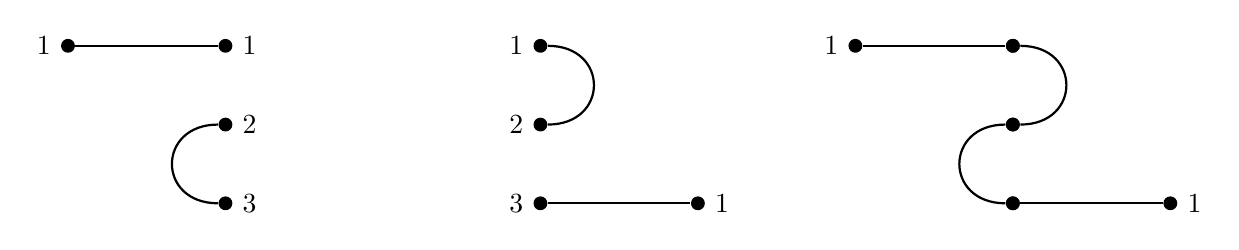
\begin{tikzpicture}
        \begin{scope}[xshift=-2cm]
            \node[circle, fill, minimum size=5pt, inner sep=0pt, label=left:{$1$}] (al1) at (-2,0) {};
            \node[circle, fill, minimum size=5pt, inner sep=0pt, label=right:{$1$}] (ar1) at (0,0) {};
            \node[circle, fill, minimum size=5pt, inner sep=0pt, label=right:{$2$}] (ar2) at (0,-1) {};
            \node[circle, fill, minimum size=5pt, inner sep=0pt, label=right:{$3$}] (ar3) at (0,-2) {};
                \draw[thick] (al1) to (ar1);
                \draw[thick, out=180, in=180, looseness=2] (ar2) to (ar3);
        \end{scope}
        \begin{scope}[xshift=2cm]
            \node[circle, fill, minimum size=5pt, inner sep=0pt, label=right:{$1$}] (br3) at (2,-2) {};
            \node[circle, fill, minimum size=5pt, inner sep=0pt, label=left:{$1$}] (bl1) at (0,0) {};
            \node[circle, fill, minimum size=5pt, inner sep=0pt, label=left:{$2$}] (bl2) at (0,-1) {};
            \node[circle, fill, minimum size=5pt, inner sep=0pt, label=left:{$3$}] (bl3) at (0,-2) {};
                \draw[thick, out=0, in=0, looseness=2] (bl1) to (bl2);
                \draw[thick] (bl3) to (br3);
        \end{scope}
        \begin{scope}[xshift=8cm]
            \begin{scope}[xshift=-0cm]
                \node[circle, fill, minimum size=5pt, inner sep=0pt,label=left:{$1$}] (al1) at (-2,0) {};
                \node[circle, fill, minimum size=5pt, inner sep=0pt] (ar1) at (0,0) {};
                \node[circle, fill, minimum size=5pt, inner sep=0pt] (ar2) at (0,-1) {};
                \node[circle, fill, minimum size=5pt, inner sep=0pt] (ar3) at (0,-2) {};
                    \draw[thick] (al1) to (ar1);
                    \draw[thick, out=180, in=180, looseness=2] (ar2) to (ar3);
            \end{scope}
            \begin{scope}[xshift=0cm]
                \node[circle, fill, minimum size=5pt, inner sep=0pt, label=right:{$1$}] (br3) at (2,-2) {};
                \node[circle, fill, minimum size=5pt, inner sep=0pt] (bl1) at (0,0) {};
                \node[circle, fill, minimum size=5pt, inner sep=0pt] (bl2) at (0,-1) {};
                \node[circle, fill, minimum size=5pt, inner sep=0pt] (bl3) at (0,-2) {};
                    \draw[thick, out=0, in=0, looseness=2] (bl1) to (bl2);
                    \draw[thick] (bl3) to (br3);
            \end{scope}
        \end{scope}
    \end{tikzpicture}}
\end{equation*}
%
Indeed, there is a bicategory $\catopengrph$ that has sets as objects, open graphs as morphisms, and interface-preserving graph homomorphisms as 2-morphisms.
For instance, the first and second open graphs above correspond to morphisms $G\colon \{1\} \to \{1,2,3\}$ and $H\colon \{1,2,3\} \to \{1\}$. 
These morphisms can be composed, resulting in the morphism $G \Cp H\colon \{1\} \to \{1\}$ corresponding to the third open graph in the picture above.

Every graph can be mapped to its \emph{reachability relation}\footnote{Cfr. \cite{lorenz2023causal}, for the similar example of open causal models and causal influence.}: this is a relation on the vertexes of the graph, where two vertexes are considered related iff there is a path between them.
Reachability can be recast as a lax functor $\catopengrph \to \catrel$ to the bicategory of sets, relations, and inclusions of relations, which maps an open graph $G\colon X \to Y$ to the relation $\fun{R}G\colon X \to Y$ defined by
\begin{equation*}
    \text{$\fun{R}G(x, y)$ if and only if there is a path between the input vertex $x$ and the output vertex $y$.}
\end{equation*}
Because $\catrel$ is locally posetal, to define $\fun{R}$ on 2-morphisms it suffices to verify that, if $f\colon G \to G'$ is a graph homomorphism, then $\fun{R}G \subseteq \fun{R}G'$.
The laxators are also uniquely defined.

We can see that this functor is not strong.
In the example above we have that $\fun{R}G \subseteq \{1\} \times \{1,2,3\}$ only contains the pair $(1,1)$, since there are no paths from $1$ to $2$ and from $1$ to $3$ in $G$.
Similarly, $\fun{R}H \subseteq \{1,2,3\} \times \{1\}$ only contains the pair $(3,1)$.
It follows that $\fun{R}G \Cp \fun{R}H\colon \{1\} \to \{1\}$ is the empty relation, but $\fun{R}(G \Cp H)\colon \{1\} \to \{1\}$ is total, so $\fun{R}G \Cp \fun{R}H \subsetneq \fun{R}(G \Cp H)$.

The result is that, if we want to compute the reachability relation of $G \Cp H$ by looking at the reachability relations of $G$ and $H$ separately, we are going to miss something.
This ``compositionality gap'' is tracked by the $\pi_0$ associated to the laxator components $\varphi_{G, H}\colon \fun{R}G \Cp \fun{R}H \subseteq \fun{R}(G \Cp H)$ (because these are all injective, the $\pi_1$ will always be trivial).

In our example, $\dhom{0}{(\slice{\homset{\catrel}{\{1\}}{\{1\}}}{\fun{R}(G\Cp H)})}{\varphi_{G,H}}$ is isomorphic to the poset $(\varnothing < \{(1, 1)\})$ pointed with $\varnothing$, so there is exactly one non-trivial obstruction.
Using covariance, we can think of ``removing the obstruction'' by modifying one or both of the parts $G$ or $H$ with a 2-morphism, that is, with a graph homomorphism.
For example, we can act on $G$ with the homomorphism which identifies the output vertices $1$ and $3$.
The resulting graph $G'$ has $\fun{R}G' = \{(1, 1), (1, 3)\}$, so $\fun{R}G' \Cp \fun{R}H = \fun{R}(G' \Cp H) = \{(1, 1)\}$; correspondingly, we obtain a map of pointed posets from the $\pi_0$ associated to $\varphi_{G, H}$ to the $\pi_0$ associated to $\varphi_{G', H}$, which ``trivialises all obstructions''.
%
%
\subsection{Schr\"odinger Compositionality}\label{subsec: schrodinger compositionality}

The name \emph{Schr\"odinger compositionality} was introduced in \cite{coecke2021compositionality} to refer to the form of compositionality that exists in quantum mechanics, where \emph{non-separable states} are present, to disambiguate it from others.
\footnote{For the purposes of this work, we are leaving out of the present analysis the aspects of Schr\"odinger compositionality regarding the  ``ontological interpretation", originally presented in  \cite{coecke2021compositionality}.}
%One key implication of Schr\"odinger compositionality is that ``a state can be more than its parts''.
In the following, we will focus on the special case of a state that can be ``more than its parts''.
This is arguably what makes composition interesting in quantum mechanics: it makes entanglement possible, which Schr\"odinger described as ``the characteristic trait of quantum mechanics'' \cite{Schrodinger_1935}.
In contrast with the example of open graphs, where the ``compositionality gap'' represents an obstacle to a computation strategy, here it can be seen as a positive feature.
Our approach can be used in both contexts; we will focus on the case study of non-separable states, recasting it as the failure of a lax functor to be strong.

In the context of monoidal categories,
%\footnote{Technically, thoughout the section we implicitly assume that our monoidal categories are strict. The example can easily be reworked for general monoidal categories by introducing unitors where it is suitable.}
a \emph{state} is a morphism $\TensorUnit \to A$, where $\TensorUnit$ is the monoidal unit.
We say that a state $\psi\colon \TensorUnit \to A \otimes B$ is \emph{separable} if there exist states $\psi_A\colon \TensorUnit \to A$ and $\psi_B\colon \TensorUnit \to B$ such that $\psi = \psi_A \otimes \psi_B$.%\footnote{Note that we are referring here to the notion of separability of pure states.}, or, graphically:
%
%
%\begin{equation*}
    %\begin{tikzpicture}
     %   \node[draw,thick,minimum width=2cm, minimum height=0.75cm] (phiAB) at (0,0) {$\psi$};
      %      \draw[thick] ($(phiAB.north) - (0.5,0)$) -- +(0,0.75);
       %     \draw[thick] ($(phiAB.north) + (0.5,0)$) -- +(0,0.75);
       % \node (equals) at (1.75,0) {$=$};
       % \node[draw,thick,minimum width=1cm, minimum height=2] (phiA) at (3,0) {$\psi_{A}$};
       %     \draw[thick] (phiA.north) -- +(0,0.75);
       % \node[draw,thick,minimum width=1cm, minimum height=2] (phiB) at (4.5,0) {$\psi_{B}$};
       %     \draw[thick] (phiB.north) -- +(0,0.75);
    %\end{tikzpicture}
%\end{equation*}
%

%
%
\begin{definition}
    Let $(\cat{C}, \otimes, \TensorUnit)$ be a monoidal category.
    The \emph{state functor} of $\cat{C}$ is the representable functor $\homset{\cat{C}}{\TensorUnit}{-}\colon \cat{C} \to \catset$. 
\end{definition}
%
\begin{proposition}[Laxity of the state functor]\label{prop: state functor lax}
    The state functor lifts to a lax monoidal functor from $(\cat{C}, \otimes, \TensorUnit)$ to $(\catset, \times, \{*\})$, with laxator components
    \begin{align*}
        \varphi_{A,B}\colon \homset{\CategoryC}{\TensorUnit}{A} \times \homset{\CategoryC}{\TensorUnit}{B}
            &\rightarrow 
            \homset{\CategoryC}{\TensorUnit}{A \otimes B}\\
        (\psi_A, \psi_B) 
            &\mapsto
            \psi_A \otimes \psi_B.
    \end{align*}
\end{proposition}
%
%
Recall that a monoidal category is \emph{semicartesian} if its monoidal unit is terminal.
The following result is a consequence of the general fact that a functor from a semicartesian to a cartesian monoidal category has a canonical oplax monoidal structure.
%
%
\begin{proposition}[Oplaxity of the state functor]\label{prop: state functor oplax}
    Let $(\cat{C}, \otimes, \Term)$ be a semicartesian category.
    Then the state functor lifts to an oplax monoidal functor from $(\cat{C}, \otimes, \Term)$ to $(\catset, \times, \{*\})$.
\end{proposition}
%
Clearly, there are cases where the state functor is not just lax or oplax, but strong.
The following result captures the well-known fact that in a cartesian monoidal category every state is separable.
%
\begin{proposition}[Strongness of the state functor]\label{prop: state functor strong}
    If $(\CategoryC, \times, \Term)$ is cartesian, then the state functor is strong monoidal.
\end{proposition}

Having turned Schr\"odinger compositionality into a question about (op)laxity of a functor, we can put our framework to good work.
By \autoref{prop: covariance natural transformation}, we have functors $\cat{C} \times \cat{C} \to \pointed{\catpos}$ sending pairs of objects $(A, B)$ of $\cat{C}$ to the homotopy posets 
\begin{equation} \label{eq: state_dhom }
    \dhom{i}{(\slice{\Set}{\homset{\cat{C}}{I}{A \otimes B}})}{\varphi_{A, B}}, \quad i \in \{ 0, 1 \}.
\end{equation}
Using the description of homotopy posets for slices of $\Set$ from \autoref{sec: obstructions}, we see that
\begin{itemize}
    \item minimal obstructions in $\pi_0$ are in bijection with non-separable states of $A \otimes B$,
    \item minimal obstructions in $\pi_1$ are in bijection with pairs of pairs of states $((\psi_A, \psi_B), (\chi_A, \chi_B))$ such that $\psi_A \otimes \psi_B = \chi_A \otimes \chi_B$.
\end{itemize}
For example, in $(\lcat{Vect}_\mathbb{C}, \otimes, \mathbb{C})$, the monoidal category of complex vector spaces with their tensor product, whenever $A$ and $B$ are at least 2-dimensional, we have instances of both:
\begin{itemize}
    \item the state $1 \mapsto \begin{pmatrix}1 \\ 0\end{pmatrix} \otimes \begin{pmatrix}1 \\ 0\end{pmatrix} + \begin{pmatrix}0 \\ 1\end{pmatrix} \otimes \begin{pmatrix}0 \\ 1\end{pmatrix}$ of $\mathbb{C}^2 \otimes \mathbb{C}^2$ is non-separable,
    \item given any pair of states $(\psi_A, \psi_B)$ and any non-zero $\lambda \in \mathbb{C}$, the pair $(\chi_A, \chi_B) \eqdef (\lambda \psi_A, \invrs{\lambda} \psi_B)$ satisfies $\psi_A \otimes \psi_B = \chi_A \otimes \chi_B$.
\end{itemize}
We can derive a few simple, immediate consequences from the covariance of (\ref{eq: state_dhom }) in the pair $(A, B)$.
\begin{enumerate}
    \item Given morphisms $f\colon A \to A'$, $g\colon B \to B'$, the induced maps of posets preserve the basepoint, that is, map ``non-obstructions'' to ``non-obstructions''.
    In this case, this implies that \emph{it is not possible to entangle a separable state by local actions}, that is, by applying morphisms on $A$ and $B$ separately.
    \item On the other hand, it is, in principle, possible for the induced maps to send non-trivial obstructions to the basepoint.
    For example, in complex vector spaces, acting on $A$ or $B$ with a rank-1 linear map always has a separating effect.
\end{enumerate}

    \section{Future work}
\label{sec:future-work}

In conclusion we discuss several directions for further work.

One is to explore how Clerical could be extended to include higher-order functions and general recursion.
%
Incorporating higher-order function without recursion should be straightforward from a language-design viewpoint. However, generalising the denotational semantics to cover higher-order functions may not be so straightforward, since the powerdomain $\PP{S}$ from 
Section~\ref{sec:denotation} will have to be generalised to allow $S$ to range over denotations of arbitrary types. 
%
With regards to general recursion, the non-monotonicity phenomena associated with the guarded case construct are likely to make it very challenging to define denotational semantics; see~\cite{LEVY2007221} for a discussion of related issues.

Second, in this paper we have not presented any formal operational semantics for Clerical.
Having one would provide an alternative and direct
account of the computability of the language, as well as a
framework within which implementation-relevant information, such as
the scope for parallelism in the execution strategy, could be studied in a mathematical setting. Also, a formally specified operational semantics
could guide implementations of Clerical and Clerical-like languages, and help estaliblish their correctness.

Third, we could further experiment with our implementation, which is good enough to evaluate the~$\pi$ program but cannot compete with the mature libraries for exact-real numbers.
%
To speed it up, we should at least implement parallel execution of threads, which is supported by the latest OCaml version.
%
A more substantive improvements would explore better evaluation strategies for nondeterminism, and compilation to a more efficient low-level language.

Fourth, there is significant room for improvement in the Coq formalization. By implementing better automation and tactics for proving correctness assertions, we would obtain a workable environment for formal verification of exact real computation, supported by the formidable machinery of Coq.

	\nocite{*}
	\begin{raggedright}
	\bibliographystyle{eptcs}
	\bibliography{main}
	\end{raggedright}
	
    \begin{partbacktext}
\part{Appendices}
\end{partbacktext}

\appendix

\chapter{Collections}
\label{appendix:collections}

\abstract{This appendix gives a description of the vector collections used in experiments
throughout this monograph. These collections demonstrate different operating points in
a typical use-case. For example, some consist of dense vectors, others of sparse vectors;
some have few dimensions and others are in much higher dimensions; some are relatively small
while others contain a large number of points.}

\bigskip

Table~\ref{table:appendix:collections:dense} gives a description of the dense vector collections
used throughout this monograph and summarizes their key statistics.

\begin{table*}[ht]
\caption{Dense collections used in this monograph along with select statistics.}
\scriptsize
\label{table:appendix:collections:dense}
\begin{center}
\begin{sc}
\begin{tabular}{p{5cm}|ccc}
\toprule
Collection & Vector Count & Query Count & Dimensions \\
\midrule
\textsc{GloVe}-$25$~\citep{pennington-etal-2014-glove} & $1.18$M & $10{,}000$ & $25$ \\
\textsc{GloVe}-$50$ & $1.18$M & $10{,}000$ & $50$ \\
\textsc{GloVe}-$100$ & $1.18$M & $10{,}000$ & $100$ \\
\textsc{GloVe}-$200$ & $1.18$M & $10{,}000$ & $200$ \\
\textsc{Deep1b}~\citep{deep1b} & $9.99$M & $10{,}000$ & $96$ \\
\textsc{MS Turing}~\citep{msturingDataset} & $10$M & $100{,}000$ & $100$ \\
\textsc{Sift}~\citep{Lowe2004DistinctiveIF} & $1$M & $10{,}000$ & $128$ \\
\textsc{Gist}~\citep{Oliva2001ModelingTS} & $1$M & $1{,}000$ & $960$ \\
\bottomrule
\end{tabular}
\end{sc}
\end{center}
\end{table*}

In addition to the vector collections above, we convert a few text collections
into vectors using various embedding models. These collections are described in
Table~\ref{table:appendix:collections:text}. Please see~\citep{nguyen2016msmarco} for
a complete description of the MS MARCO v1 collection and~\citep{thakur2021beir} for the others.

\begin{table*}[ht]
\caption{Text collections along with key statistics.
The rightmost two columns report the average number of non-zero
entries in data points and, in parentheses, queries for sparse vector
representations of the collections.}
\scriptsize
\label{table:appendix:collections:text}
\begin{center}
\begin{sc}
\begin{tabular}{c|cc|cc}
\toprule
Collection & Vector Count & Query Count & \splade{} & \esplade{}\\
\midrule
\textsc{MS Marco} Passage& $8.8$M & $6{,}980$ & 127 (49) & 185 (5.9) \\
NQ & $2.68$M & $3{,}452$ & 153 (51) & 212 (8) \\
\textsc{Quora} & $523$K & $10{,}000$ & 68 (65) & 68 (8.9) \\
\textsc{HotpotQA} & $5.23$M & $7{,}405$ & 131 (59) & 125 (13) \\
\textsc{Fever} & $5.42$M & $6{,}666$ & 145 (67) & 140 (8.6) \\
\textsc{DBPedia} & $4.63$M & $400$ & 134 (49) & 131 (5.9) \\
\bottomrule
\end{tabular}
\end{sc}
\end{center}
\end{table*}

When transforming the text collections of Table~\ref{table:appendix:collections:text}
into vectors, we use the following embedding models:
\begin{itemize}
    \item \textsc{AllMiniLM-l6-v2}:\footnote{Available at \url{https://huggingface.co/sentence-transformers/all-MiniLM-L6-v2}}
    Projects text documents into $384$-dimensional dense vectors for retrieval with angular distance.

    \item \textsc{Tas-B}~\citep{tas-b}: A bi-encoder model that was trained using supervision from a cross-encoder and a ColBERT~\citep{colbert2020khattab} model,
    and produces $768$-dimensional dense vectors that are meant for MIPS.
    The checkpoint used in this work is available on HuggingFace.\footnote{Available at \url{https://huggingface.co/sentence-transformers/msmarco-distilbert-base-tas-b}}

    \item \splade{}~\citep{formal2022splade}:\footnote{Pre-trained checkpoint from HuggingFace available at \url{https://huggingface.co/naver/splade-cocondenser-ensembledistil}}
    Produces sparse representations for text.
    The vectors have roughly $30{,}000$ dimensions, where each dimension corresponds
    to a term in the BERT~\citep{devlin2019bert} WordPiece~\citep{wordpiece} vocabulary.
    Non-zero entries in a vector reflect learnt term importance weights.

    \item \esplade{}~\citep{lassance2022sigir}:\footnote{Pre-trained checkpoints for document and
    query encoders were obtained from \url{https://huggingface.co/naver/efficient-splade-V-large-doc} and \url{https://huggingface.co/naver/efficient-splade-V-large-query},
    respectively.}
    This model produces queries that have far fewer non-zero entries than the original
    \splade{} model, but documents that may have a larger number of non-zero entries.
\end{itemize}

\bibliographystyle{abbrvnat}
\bibliography{biblio}


\chapter{Probability Review}
\label{appendix:probability}

\abstract{We briefly review key concepts in probability in this appendix.}

\section{Probability}
We identify a \emph{probability space} denoted by $(\Omega, \mathcal{F}, \probability)$
with an \emph{outcome space}, an \emph{events} set, and a \emph{probability measure}.
The outcome space, $\Omega$, is the set of all
possible outcomes. For example, when flipping a two-sided coin, the outcome
space is simply $\{0, 1\}$. When rolling a six-sided die, it is instead
the set $[6] = \{ 1, 2, \ldots, 6\}$.

The events set $\mathcal{F}$ is a set of subsets of $\Omega$ that
includes $\Omega$ as a member and is closed under complementation and
countable unions. That is, if $E \in \mathcal{F}$,
then we must have that $E^\complement \mathcal{F}$.
Furthermore, the union of countably many events $E_i$'s
in $\mathcal{F}$ is itself in $\mathcal{F}$: $\cup_i E_i \in \mathcal{F}$.
A set $\mathcal{F}$ that satisfies these properties is called a $\sigma$-algebra.

Finally, a function $\probability: \mathcal{F} \rightarrow \mathbb{R}$ is
a probability measure if it satisfies the following conditions: $\probability[\Omega] = 1$;
$\probability[E] \geq 0$ for any event $E \in \mathcal{F}$;
$\probability[E^\complement] = 1 - \probability[E]$; and, finally,
for countably many disjoint events $E_i$'s:
$\probability[\cup_i E_i] = \sum_i \probability[E_i]$.

We should note that, $\probability$ is also known as a ``probability distribution''
or simply a ``distribution.'' The pair $(\Omega, \mathcal{F})$ is called
a \emph{measurable space}, and the elements of $\mathcal{F}$ are
known as a \emph{measurable sets}. The reason they are called ``measurable''
is because they can be ``measured'' with $\probability$: The function
$\probability$ assigns values to them.

In many of the discussions throughout this monograph, we omit the outcome space
and events set because that information is generally clear from context.
However, a more formal treatment of our arguments requires a complete
definition of the probability space.

\section{Random Variables}
A random variable on a measurable space $(\Omega, \mathcal{F})$ is
a measurable function $X: \Omega \rightarrow \mathbb{R}$.
It is measurable in the sense that the \emph{preimage} of any Borel set $B \in \mathcal{B}$
is an event: $X^{-1}(B) = \{ \omega \in \Omega \;|\; X(\omega) \in B \} \in \mathcal{F}$.

A random variable $X$ generates a $\sigma$-algebra that comprises of the preimage
of all Borel sets. It is denoted by $\sigma(X)$
and formally defined as $\sigma(X) = \{ X^{-1}(B) \;|\; B \in \mathcal{B} \}$.

\bigskip

Random variables are typically categorized as discrete or continuous.
$X$ is \emph{discrete} when it maps $\Omega$ to a discrete set.
In that case, its \emph{probability mass function} is defined as $\probability[X = x]$
for some $x$ in its range.
A \emph{continuous} random variable is often associated with a
probability \emph{density} function, $f_X$, such that:
\begin{equation*}
    \probability[a \leq X \leq b] = \int_a^b f_X(x) dx.
\end{equation*}

Consider, for instance, the following probability density function over the real line for
parameters $\mu \in \mathbb{R}$ and $\sigma > 0$:
\begin{equation*}
    f(x) = \frac{1}{\sqrt{2 \pi \sigma^2}} e^{- \frac{(x - \mu)^2}{2\sigma^2}}.
\end{equation*}
A random variable with the density function above is said to follow a Gaussian
distribution with mean $\mu$ and variance $\sigma^2$, denoted by $X \sim \mathcal{N}(\mu, \sigma^2)$.
When $\mu = 0$ and $\sigma^2 = 1$, the resulting distribution is called the standard
Normal distribution.

Gaussian random variables have attractive properties.
For example, the sum of two independent Gaussian random variables is itself a Gaussian variable.
Concretely, $X_1 \sim \mathcal{N}(\mu_1, \sigma_1^2)$ and $X_2 \sim \mathcal{N}(\mu_2, \sigma_2^2)$,
then $X_1 + X_2 \sim \mathcal{N}(\mu_1 + \mu_2, \sigma_1^2 + \sigma_2^2)$.
The sum of the squares of $m$ independent Gaussian random variables, on the other hand,
follows a $\chi^2$-distribution with $m$ degrees of freedom.

\section{Conditional Probability}
Conditional probabilities give us a way to model how the probability of an event changes
in the presence of extra information, such as partial knowledge about a random outcome.
Concretely, if $(\Omega, \mathcal{F}, \probability)$ is a probability space and
$A, B \in \mathcal{F}$ such that $\probability[B] > 0$, then the \emph{conditional
probability} of $A$ given the event $B$ is denoted by $\probability[A \;\lvert\; B]$ and
defined as follows:
\begin{equation*}
    \probability[A \;\lvert\; B] = \frac{\probability[A \cap B]}{\probability[B]}.
\end{equation*}

We use a number of helpful results concerning conditional probabilities
in proofs throughout the monograph. One particularly useful inequality
is what is known as the \emph{union bound} and is stated as follows:
\begin{equation*}
    \probability[\cup_i A_i] \leq \sum_i \probability[A_i].
\end{equation*}

Another fundamental property is the law of total probability.
It states that, for mutually disjoint events $A_i$'s such that
$\Omega = \cup A_i$, the probability of any event $B$ can be expanded
as follows:
\begin{equation*}
    \probability[B] = \sum_i \probability[B \;\lvert\; A_i] \probability[A_i].
\end{equation*}
This is easy to verify: the summand is by definition equal to $\probability[B \cap A_i]$
and, considering the events $(B \cap A_i)$'s are mutually disjoint, their sum
is equal to $\probability[B \cap (\cup A_i)] = \probability[B]$.


\section{Independence}
Another tool that reflects the effect (or lack thereof) of additional knowledge on probabilities
is the concept of \emph{independence}. Two events $A$ and $B$ are said to be
\emph{independent} if $\probability[A \cap B] = \probability[A] \times \probability[B]$.
Equivalently, we say that $A$ is independent of $B$ if and only if
$\probability[A \;\lvert\; B] = \probability[A]$ when $\probability[B] > 0$.

\bigskip

Independence between two random variables is defined similarly but requires a bit more care.
If $X$ and $Y$ are two random variables and $\sigma(X)$ and $\sigma(Y)$ denote
the $\sigma$-algebras generated by them, then $X$ is independent of $Y$ if
all events $A \in \sigma(X)$ and $B \in \sigma(Y)$ are independent.

When a sequence of random variables are \emph{mutually} independent and are drawn
from the same distribution (i.e., have the same probability density function),
we say the random variables are drawn \emph{iid}: independent and identically-distributed.
We stress that \emph{mutual} independence is a stronger restriction than
\emph{pairwise} independence: $m$ events $\{ E_i \}_{i=1}^m$ are mutually independent if
$\probability[\cap_i E_i] = \prod_i \probability[E_i]$.

We typically assume that data and query points are drawn \emph{iid} from some
(unknown) distribution. This is a standard and often necessary assumption
that eases analysis.

\section{Expectation and Variance}

The \emph{expected value} of a discrete random variable $X$ is denoted by $\ev[X]$
and defined as follows:
\begin{equation*}
    \ev[X] = \sum_x x \probability[X = x].
\end{equation*}
When $X$ is continuous, its expected value is based on the following Lebesgue integral:
\begin{equation*}
    \ev[X] = \int_{\Omega} X d \probability.
\end{equation*}
So when a random variable has probability density function $f_X$, its expected value
becomes:
\begin{equation*}
    \ev[X] = \int x f_X(x) dx.
\end{equation*}

For a \emph{nonnegative} random variable $X$, it is sometimes more convenient to
unpack $\ev{X}$ as follows instead:
\begin{equation*}
    \ev[X] = \int_0^\infty \probability[X > x] dx.
\end{equation*}

A fundamental property of expectation is that it is a linear operator.
Formally, $\ev[X + Y] = \ev[X] + \ev[Y]$ for two random variables $X$ and $Y$.
We use this property often in proofs.

We state another important property for independent random variables
that is easy to prove.
If $X$ and $Y$ are independent, then $\ev[XY] = \ev[X]\ev[Y]$.

\bigskip

The \emph{variance} of a random variable is defined as follows:
\begin{equation*}
    \var[X] = \ev\Big[ (X - \ev[X])^2 \Big] = \ev[X]^2 - \ev[X^2].
\end{equation*}
Unlike expectation, variance is not linear unless the random variables involved
are independent. It is also easy to see that $\var[aX] = a^2 \var[X]$ for a
constant $a$.

\section{Central Limit Theorem}
The result known as the Central Limit Theorem is one of the most
useful tools in probability. Informally, it states that the average of \emph{iid}
random variables with finite mean and variance converges to a Gaussian distribution.
There are several variants of this result that extend the claim to, for example,
independent but not identically distributed variables. Below we repeat the formal
result for the \emph{iid} case.

\begin{theorem}
    Let $X_i$'s be a sequence of $n$ \emph{iid} random variables with finite mean $\mu$
    and variance $\sigma^2$. Then, for any $x \in \mathbb{R}$:
    \begin{equation*}
        \lim_{n \rightarrow \infty} \probability \Big[
            \underbrace{\frac{(1/n \sum_{i=1}^n X_i) - \mu}{\sigma^2/n}}_Z \leq x
        \Big] = \int_{-\infty}^x \frac{1}{\sqrt{2 \pi}} e^{-\frac{t^2}{2}} dt,
    \end{equation*}
    implying that $Z \sim \mathcal{N}(0, 1)$.
\end{theorem}

\chapter{Concentration of Measure}
\label{appendix:measure}

\abstract{
By the strong law of large numbers, we know that the average of a sequence
of $m$ \emph{iid} random variables with mean $\mu$ converges to $\mu$ with
probability $1$ as $m$ tends to infinity. But how far is that average from
$\mu$ when $m$ is finite? Concentration inequalities helps us answer that question
quantitatively. This appendix reviews important inequalities that are used
in the proofs and arguments throughout this monograph.
}

\section{Markov's Inequality}

\begin{lemma}
    \label{lemma:appendix:concentration:markov}
    For a nonnegative random variable $X$ and a nonnegative constant $a \geq 0$:
    \begin{equation*}
        \probability[X \geq a] \leq \frac{\ev[X]}{a}.
    \end{equation*}
\end{lemma}
\begin{proof}
    Recall that the expectation of a nonnegative random variable $X$ can be written
    as:
    \begin{equation*}
        \ev[X] = \int_0^\infty \probability[X \geq x] dx.
    \end{equation*}
    Because $\probability[X \geq x]$ is monotonically nonincreasing, we can expand
    the above as follows to complete the proof:
    \begin{equation*}
        \ev[X] \geq \int_0^a \probability[X \geq x] dx \geq \int_0^a \probability[X \geq a] dx = a \probability[X \geq a].
    \end{equation*}
\end{proof}

\section{Chebyshev's Inequality}

\begin{lemma}
    \label{lemma:appendix:concentration:chebyshev}
    For a random variable $X$ and a constant $a > 0$:
    \begin{equation*}
        \probability \Big[ \big\lvert X - \ev[X] \big\rvert \geq a \Big] \leq \frac{\var[X]}{a^2}.
    \end{equation*}
\end{lemma}
\begin{proof}
    \begin{equation*}
        \probability \Big[ \big\lvert X - \ev[X] \big\rvert \geq a \Big] =
        \probability \Big[ \big( X - \ev[X] \big)^2 \geq a^2 \Big] \leq \frac{\var[X]}{a^2},
    \end{equation*}
    where the last step follows by the application of Markov's inequality.
\end{proof}

\begin{lemma}
    Let $\{ X_i \}_{i=1}^n$ be a sequence of iid random variables
    with mean $\mu < \infty$ and variance $\sigma^2 < \infty$. For $\delta \in (0, 1)$,
    with probability $1 - \delta$:
    \begin{equation*}
        \Big\lvert \frac{1}{n} \sum_{i = 1}^n X_i - \mu \Big\rvert \leq \sqrt{\frac{\sigma^2}{\delta n}}.
    \end{equation*}
\end{lemma}
\begin{proof}
    By Lemma~\ref{lemma:appendix:concentration:chebyshev}, for any $a > 0$:
    \begin{equation*}
        \probability \Bigg[ \Big\lvert \frac{1}{n}\sum_{i=1}^n X_i - \mu \Big\rvert \geq a \Bigg]
        \leq \frac{\sigma^2/n}{a^2}.
    \end{equation*}
    Setting the right-hand-side to $\delta$, we obtain:
    \begin{equation*}
        \frac{\sigma^2}{n a^2} = \delta \implies a = \sqrt{\frac{\sigma^2}{\delta n}},
    \end{equation*}
    which completes the proof.
\end{proof}

\section{Chernoff Bounds}

\begin{lemma}
    Let $\{ X_i \}_{i=1}^n$ be independent Bernoulli variables with success probability $p_i$.
    Define $X = \sum_i X_i$ and $\mu = \ev[X] = \sum_i p_i$. Then:
    \begin{equation*}
        \probability \Big[ X > (1 + \delta) \mu \Big] \leq e^{-h(\delta) \mu},
    \end{equation*}
    where,
    \begin{equation*}
        h(t) = (1 + t) \log(1 + t) - t.
    \end{equation*}
\end{lemma}
\begin{proof}
    Using Markov's inequality of Lemma~\ref{lemma:appendix:concentration:markov}
    we can write the following for any $t > 0$:
    \begin{equation*}
        \probability\Big[ X > (1 + \delta)\mu \Big] =
            \probability\Big[ e^{tX} > e^{t(1 + \delta)\mu} \Big] \leq
            \frac{\ev\big[ e^{tX} \big]}{e^{t (1 + \delta) \mu}}.
    \end{equation*}
    Expanding the expectation, we obtain:
    \begin{align*}
        \ev\big[e^{tX}\big] &= \ev\Big[ e^{t \sum_i X_i} \Big] = \ev\Big[ \prod_i e^{tX_i} \Big]
        = \prod_i \ev[e^{tX_i}] \\
        &= \prod_i \Big( p_i e^t + (1 - p_i) \Big) \\
        &= \prod_i \big( 1 + p_i (e^t - 1) \big) \\
        &\leq \prod_i e^{p_i(e^t - 1)} = e^{(e^t - 1)\mu}. && \text{by $(1 + t \leq e^t)$} \\
    \end{align*}
    Putting all this together gives us:
    \begin{equation}
        \label{equation:appendix:concentration:chernoff:proof}
        \probability\Big[ X > (1 + \delta)\mu \Big] \leq 
        \frac{e^{(e^t - 1) \mu}}{e^{t (1 + \delta) \mu}}.
    \end{equation}
    This bound holds for any value $t > 0$, and in particular a value of $t$ that
    minimizes the right-hand-side. To find such a $t$, we may differentiate
    the right-hand-side, set it to $0$, and solve for $t$ to obtain:
    \begin{align*}
        \frac{\mu e^t e^{(e^t - 1) \mu}}{e^{t (1 + \delta) \mu}} &-
        \mu ( 1 + \delta ) \frac{e^{(e^t - 1) \mu}}{e^{t (1 + \delta) \mu}} = 0 \\
        &\implies \mu e^t = \mu (1 + \delta) \\
        &\implies t = \log(1 + \delta).
    \end{align*}
    Substituting $t$ into Equation~(\ref{equation:appendix:concentration:chernoff:proof})
    gives the desired result.
\end{proof}

\section{Hoeffding's Inequality}

We need the following result, known as Hoeffding's Lemma, to present
Hoeffding's inequality.

\begin{lemma}
    \label{lemma:appendix:concentration:hoeffding-lemma}
    Let $X$ be a zero-mean random variable that takes values in $[a, b]$.
    For any $t > 0$:
    \begin{equation*}
        \ev\big[ e^{tX} \big] \leq \exp\Big( \frac{t^2 (b - a)^2}{8} \Big).
    \end{equation*}
\end{lemma}
\begin{proof}
    By convexity of $e^{tx}$ and given $x \in [a, b]$ we have that:
    \begin{equation*}
        e^{tx} \leq \frac{b - x}{b - a} e^{ta} +
            \frac{x - a}{b - a} e^{tb}.
    \end{equation*}
    Taking the expectation of both sides, we arrive at:
    \begin{equation*}
        \ev\Big[e^{tx}\Big] \leq
            \frac{b}{b - a} e^{ta} - \frac{a}{b - a} e^{tb}.
    \end{equation*}
    To conclude the proof, we first write the right-hand-side as
    $\exp(h(t(b - a)))$ where:
    \begin{equation*}
        h(x) = \frac{a}{b - a} x + \log \Big( \frac{b}{b - a} - \frac{a}{b - a} e^x \Big).
    \end{equation*}
    By expanding $h(x)$ using Taylor's theorem, it can be shown that
    $h(x) \leq x^2/8$. That completes the proof.
\end{proof}

We are ready to present Hoeffding's inequality.

\begin{lemma}
    Let $\{ X_i \}_{i=1}^n$ be a sequence of iid random variables
    with finite mean $\mu$ and suppose $X_i \in [a, b]$ almost surely.
    For all $\epsilon > 0$:
    \begin{equation*}
        \probability\Bigg[ \Big\lvert \frac{1}{n} \sum_{i=1}^n X_i - \mu \Big\rvert > \epsilon \Bigg] \leq 2 \exp\Big({-\frac{2n \epsilon^2}{(b - a)^2}}\Big).
    \end{equation*}
\end{lemma}
\begin{proof}
    Let $X = 1/n \sum_i X_i - \mu$. Observe by Markov's inequality that:
    \begin{equation*}
        \probability[X \geq \epsilon] = \probability\Big[ e^{tX} \geq e^{t\epsilon} \Big]
        \leq e^{-t\epsilon} \ev[e^{tX}].
    \end{equation*}
    By independence of $X_i$'s and
    the application of Lemma~\ref{lemma:appendix:concentration:hoeffding-lemma}:
    \begin{align*}
        \ev[e^{tX}] &= \ev \Bigg[ \prod_i e^\frac{t(X_i - \mu)}{n} \Bigg] \\
        &= \prod_i \ev \Big[ e^{\frac{t(X_i-\mu)}{n}} \Big] \\
        &\leq \prod_i \exp\Big( \frac{t^2 (b - a)^2}{8 n^2} \Big) \\
        &= \exp\Big( \frac{t^2 (b - a)^2}{8 n} \Big).
    \end{align*}
    We have shown that:
    \begin{equation*}
        \probability[X \geq \epsilon] \leq \exp\Big( -t \epsilon + \frac{t^2 (b - a)^2}{8 n} \Big).
    \end{equation*}
    That statement holds for all values of $t$ and in particular one that minimizes
    the right-hand-side. Solving for that value of $t$ gives us
    $t = 4n\epsilon / (b - a^2)$, which implies:
    \begin{equation*}
        \probability[X \geq \epsilon] \leq e^{-\frac{2n \epsilon^2}{(b - a)^2}}.
    \end{equation*}
    By a symmetric argument we can bound $\probability[X \leq -\epsilon]$. The claim
    follows by the union bound over the two cases.
\end{proof}

\section{Bennet's Inequality}

\begin{lemma}
    Let $\{ X_i \}_{i=1}^n$ be a sequence of independent random variables with zero mean
    and finite variance $\sigma_i^2$. Assume that $\lvert X_i \rvert \leq a$ almost surely for all $i$. Then:
    \begin{equation*}
        \probability\Big[\sum_i X_i \geq t \Big] \leq 
        \exp \Bigg( -\frac{\sigma^2}{a^2} h\Big( \frac{a t}{\sigma^2} \Big) \Bigg),
    \end{equation*}
    where $h(x) = (1 + x) \log(1 + x) - x$ and $\sigma^2 = \sum_i \sigma_i^2$.
\end{lemma}
\begin{proof}
    As usual, we take advantage of Markov's inequality to write:
    \begin{align*}
        \probability\Big[\sum_i X_i \geq t \Big] &\leq
            e^{-\lambda t} \ev \Big[ e^{\lambda \sum_i X_i} \Big] \\
        &= e^{-\lambda t} \ev \Big[ \prod_i e^{\lambda X_i} \Big] \\
        &= e^{-\lambda t} \prod_i \ev \Big[ e^{\lambda X_i} \Big] \\
    \end{align*}
    Using the Taylor expansion of $e^x$, we obtain:
    \begin{align*}
        \ev \Big[ e^{\lambda X_i} \Big] &= \ev \Big[ \sum_{k=0}^\infty \frac{\lambda^k X_i^k}{k!} \Big] \\
        &= 1 + \sum_{k=2}^\infty \frac{\lambda^k \ev[X_i^2 X_i^{k - 2}]}{k!} \\
        &\leq 1 + \sum_{k=2}^\infty \frac{\lambda^k \sigma_i^2 a^{k-2}}{k!} \\
        &= 1 + \frac{\sigma_i^2}{a^2} \sum_{k=2}^\infty \frac{\lambda^k a^k}{k!} \\
        &= 1 + \frac{\sigma_i^2}{a^2} \big( e^{\lambda a} - 1 - \lambda a \big) \\
        &\leq \exp\Big( \frac{\sigma_i^2}{a^2} \big( e^{\lambda a} - 1 - \lambda a \big) \Big).
    \end{align*}
    Putting it all together:
    \begin{align*}
        \probability\Big[\sum_i X_i \geq t \Big] &\leq
            e^{-\lambda t} \prod_i \exp\Big( \frac{\sigma_i^2}{a^2} \big( e^{\lambda a} - 1 - \lambda a \big) \Big) \\
        &= e^{-\lambda t} \exp\Big( \frac{\sigma^2}{a^2} \big( e^{\lambda a} - 1 - \lambda a \big) \Big).
    \end{align*}
    This inequality holds for all values of $\lambda$, and in particular one that minimizes the
    right-hand-side. Setting the derivative of the right-hand-side to $0$ and solving for $\lambda$
    leads to the desired result.
\end{proof}

\chapter{Linear Algebra Review}
\label{appendix:linear-algebra}

\abstract{
This appendix reviews basic concepts from Linear Algebra that are useful
in digesting the material in this monograph.
}

\section{Inner Product}

Denote by $\mathbb{H}$ a vector space.
An inner product $\langle \cdot, \cdot \rangle: \mathbb{H} \times \mathbb{H} \rightarrow \mathbb{R}$
is a function with the following properties:
\begin{itemize}
    \item $\forall \; u \in \mathbb{H},\; \langle u, u \rangle \geq 0$;
    \item $\forall \; u \in \mathbb{H},\; \langle u, u \rangle = 0 \Leftrightarrow u = 0$;
    \item $\forall \; u, v \in \mathbb{H},\; \langle u, v \rangle = \langle v, u \rangle$; and,
    \item $\forall \; u, v, w \in \mathbb{H}, \textit{ and } \alpha, \beta \in \mathbb{R},\; 
    \langle \alpha u + \beta v, w \rangle = \alpha \langle u, w \rangle + \beta \langle v, w \rangle$.
\end{itemize}

We call $\mathbb{H}$ together with the inner product $\langle \cdot, \cdot \rangle$
an \emph{inner product space}.
As an example, when $\mathbb{H} = \mathbb{R}^d$, given two vectors
$u = \sum_{i=1}^d u_i e_i$ and $v = \sum_{i=1}^d v_i e_i$, where $e_i$'s
are the standard basis vectors, the following is an inner product:
\begin{equation*}
    \langle u, v \rangle = \sum_{i = 1}^d u_i v_i.
\end{equation*}

We say two vectors $u$ and $v$ in an inner product space are \emph{orthogonal}
if their inner product is $0$: $\langle u, v \rangle = 0$.

\section{Norms}

A function $\Phi: \mathbb{H} \rightarrow \mathbb{R}_+$ is a norm on
$\mathbb{H}$ if it has the following properties:
\begin{itemize}
    \item Definiteness: For all $u \in \mathbb{H}$, $\Phi(u) = 0 \Leftrightarrow u = 0$;
    \item Homogeneity: For all $u \in \mathbb{H}$ and $\alpha \in \mathbb{R}$,
        $\Phi(\alpha u) = \lvert \alpha \rvert \Phi(u)$; and,
    \item Triangle inequality: $\forall \; u, v \in \mathbb{H}, \; \Phi(u + v) \leq \Phi(u) + \Phi(v)$.
\end{itemize}

Examples include the absolute value on $\mathbb{R}$,
and the $L_p$ norm (for $p \geq 1$) on $\mathbb{R}^d$ denoted by $\lVert \cdot \rVert_p$
and defined as:
\begin{equation*}
    \lVert u \rVert_p = \Big( \sum_{i=1}^d \lvert u_i \rvert^p \Big)^{\frac{1}{p}}.
\end{equation*}
Instances of $L_p$ include the commonly used $L_1$, $L_2$ (Euclidean),
and $L_\infty$ norms, where $\lVert u \rVert_\infty = \max_i \lvert u_i \rvert$.

Note that, when $\mathbb{H}$ is an inner product space, then
the function $\lVert u \rVert = \sqrt{\langle u, u \rangle}$ is a norm.

\section{Distance}
A norm on a vector space induces a notion of distance between two vectors.
Concretely, if $\mathbb{H}$ is a normed space equipped with $\lVert \cdot \rVert$,
then we define the distance between two vectors $u, v \in \mathbb{H}$ as follows:
\begin{equation*}
    \delta(u, v) = \lVert u - v \rVert.
\end{equation*}

\section{Orthogonal Projection}

\begin{lemma}
    Let $\mathbb{H}$ be an inner product space and suppose $u \in \mathbb{H}$ and $u \neq 0$.
    Any vector $v \in \mathbb{H}$ can be uniquely decomposed along $u$ as:
    \begin{equation*}
        v = v_{\perp} + v_{\parallel},
    \end{equation*}
    such that $\langle v_\perp, v_\parallel \rangle = 0$. Additionally:
    \begin{equation*}
        v_\parallel = \frac{\langle u, v \rangle}{\langle u, u \rangle} u,
    \end{equation*}
    and $v_\perp = v - v_\parallel$.
\end{lemma}
\begin{proof}
    Let $v_\parallel = \alpha u$ and $v_\perp = v - v_\parallel$.
    Because $v_\parallel$ and $v_\perp$ are orthogonal, we deduce that:
    \begin{align*}
        \langle v_\parallel, v_\perp \rangle = 0 \implies
            \langle \alpha u, v_\perp \rangle = 0 \implies
            \langle u, v_\perp \rangle = 0.
    \end{align*}
    That implies:
    \begin{align*}
        \langle v, u \rangle = \alpha \langle u, u \rangle \implies
        \alpha = \frac{\langle u, v \rangle}{\langle u, u \rangle},
    \end{align*}
    so that:
    \begin{equation*}
        v_\parallel = \frac{\langle u, v \rangle}{\langle u, u \rangle} u.
    \end{equation*}

    We prove the uniqueness of the decomposition by contradiction.
    Suppose there exists another decomposition of $v$ to $v_\parallel^\prime + v_\perp^\prime$.
    Then:
    \begin{align*}
        v_\parallel + v_\perp = v_\parallel^\prime + v_\perp^\prime &\implies
        \langle u, v_\parallel + v_\perp \rangle = \langle u,  v_\parallel^\prime + v_\perp^\prime\rangle \\
        &\implies \langle u, v_\parallel \rangle = \langle u,  v_\parallel^\prime \rangle \\
        &\implies \langle u, \alpha u \rangle = \langle u, \beta u \rangle \\
        &\implies \alpha = \beta.
    \end{align*}
    We must therefore also have that $v_\perp = v_\perp^\prime$.
\end{proof}

\end{document}
